\documentclass{note}

\course
{}
{Fall 2020}
{ETH Zürich}
{Prof. Joachim M. Buhmann and Carlos Cotrini}

\assignment
{Lecture Note: Advanced Machine Learning}
{}

\student
{Tao SUN}
{20-953-691}
{Dept. of Computer Science, ETH Z\"urich}
{taosun47@student.ethz.ch}

\setcounter{chapter}{-1}

\begin{document}
\frontmatter

\maketitle
\tableofcontents

\pagebreak

\chapter*{Acknowledgement}
This summary was made during the 2020 Fall Semester of the course \emph{Advanced Machine Learning} by Prof. Buhmann and Cotrini at ETH Z\"urich. 

The main purpose of writing this is to familiarize me with the concepts and mathematical derivations in the course. Therefore, I do not guarantee the correctness and completeness of it.

This note is mainly based on the lecture slides, tutorial materials and exercises. Some of the contents are referenced from the related books or papers. Also, some of the notes are cited from previous students, inclining @\texttt{michaelaerni}\footnote{Introduction to ML Lecture Notes, \url{https://github.com/michaelaerni/eth-introml-lecturenotes}}. The reference sources are stated in the footnotes. Many thanks to them!
	
\mainmatter

	\setcounter{page}{0}
    \pagenumbering{arabic}
    \setcounter{page}{1}
    
	\newpage
	\chapter{Math Preliminaries}
	\section{Matrix Algebra}
\subsection{Derivatives}
{\centering
\setstretch{1.3}
\begin{tabular}{p{7cm}p{7cm}}
\multicolumn{2}{c}{For $f(\bfx): \R^{n} \rightarrow \R$, $f'(\bfx) \in \R^n$ } \\  \midrule
$\diff{\bfx}(\bfb^\top \bfx) = \diff{\bfx}(\bfx^\top \bfb) = \bfb $ & $\diff{\bfx}(\bfx^\top \bfx) = 2 \bfx$ \\
$\diff{\bfx}(\norm{\bfA \bfx - \bfb}_2) = \frac{\bfA^\top (\bfA\bfx - \bfb)}{\norm{\bfA\bfx - \bfb}_2}$ & $\diff{\bfx}(\norm{\bfA \bfx - \bfb}_2^2) = {2\bfA^\top (\bfA\bfx - \bfb)}$ \\
\\
\multicolumn{2}{c}{For $f(\bfX): \R^{n \times m} \rightarrow \R$, $f'(\bfX) \in \R^{n \times m}$} \\
\midrule
$\diff{\bfX}(\bfa^\top \bfX \bfb) = \bfa \bfb^\top $ & $\diff{\bfX}(\bfa^\top \bfX^\top \bfb) = \bfb \bfa^\top $ \\
$\diff{\bfX}\mathrm{Tr}(\bfA^\top \bfX \bfB) = \bfA \bfB^\top $ & $\diff{\bfX}\mathrm{Tr}(\bfA^\top \bfX^\top \bfB) = \bfB \bfA^\top $ \\
$\diff{\bfX} |\bfX| = |\bfX| (\bfX^{-1})^\top$
\end{tabular}
}
\subsection{Inverses}
\subsubsection{Moore-Penrose Inverse}
Moore-Penrose pseudo-inverse of $\bfA \in \R^{n \times m}$ (assuming $\bfA$ has a SVD as $\bfA = \bfV \bfD \bfU^\top$):
\begin{equation}
	\bfA^+ = \left\{ (\bfA^\top \bfA)^{-1}\bfA^\top \text{ or } \bfA^\top (\bfA \bfA^\top)^{-1} \right\}= \bfV \bfD^+ \bfU^\top \in \R^{m \times n}
\end{equation}
where $ \bfD = \mathrm{diag}(\sigma_1, \cdots, \sigma_r), \bfD^+ = \mathrm{diag}(\sigma_1^{-1}, \cdots, \sigma_r^{-1}) \in \R^{r \times r}$ and $r = \mathrm{rank}(\bfA)$.

\subsubsection{Identities}
Sherman-Morrison Lemma:
\begin{equation}
\left(\mathbf{A}+\mathbf{b c}^{\top}\right)^{-1}=\mathbf{A}^{-1}-\frac{\mathbf{A}^{-1} \mathbf{b} \mathbf{c}^{\top} \mathbf{A}^{-1}}{1+\mathbf{c}^{\top} \mathbf{A}^{-1} \mathbf{b}}
\end{equation}
Woodbury Identity (and its variations):
\begin{align}
(\mathbf{A}+\mathbf{B C})^{-1} & =\mathbf{A}^{-1}-\mathbf{A}^{-1} \mathbf{B}\left(\mathbf{I}+\mathbf{C A}^{-1} \mathbf{B}\right)^{-1} \mathbf{C A}^{-1} \\
\left(\bfA+\bfU \bfC \bfV\right)^{-1} & =\bfA^{-1}-\bfA^{-1}\bfU\left(\bfC^{-1}+\bfV \bfA^{-1} \bfU\right)^{-1}\bfV \bfA^{-1}
\end{align}
\subsection{Positive-definite Matrices}
For a symmetric matrix $\bfA \in \R^{n \times n}$, 
\begin{equation}
	\bfA \mathrm{\ is\ PD}\ \Longleftrightarrow\ \bfx^\top \bfA \bfx > 0\ (\bfx \neq 0)\ \Longleftrightarrow\ \mathrm{eig}(\bfA) > 0\ \Longleftrightarrow \ \bfA = \bfB^\top \bfB \ \Longleftrightarrow \ \mathrm{ Sylvester's}.
\end{equation}
Here, \textit{Sylvester's\ criterion} is to say that all leading principal minors of $\bfA$ must be positive.

\section{Statistics and Probability}
\begin{property}[Probability Three Axioms]
\ 
\begin{enumerate}
	\item Normalization:  $p(\Omega) = 1$;
 	\item Non-negativity: $p(A) \geq 0 \ \mathrm{ for\ all }\ A \in \mathcal{F}$;
	\item $\sigma$-Additivity: $ \displaystyle \forall A_{1}, \ldots A_{n}, \ldots \in \mathcal{F} \ \mathrm{disjoint}: p\left(\bigcup_{i=1}^{\infty} A_{i}\right)=\sum_{i=1}^{\infty} p\left(A_{i}\right)$
\end{enumerate}
	\end{property}

\begin{definition}[Conditional Probability]
	\begin{equation}
p(a \mid b)=\frac{p(a \wedge b)}{p(b)}, \ \mathrm{if}\ p(b) \neq 0
\end{equation}
\end{definition}
\begin{property}[Joint Distributions]
\ \marginnote{\footnotesize Note that $x_{1:n} = x_1, x_2, \cdots, x_n$}[0cm]
\begin{enumerate}
	\item Sum Rule (a.k.a Marginalization) \begin{equation}
p\left(X_{i}\right)=\sum_{x_{1}, \ldots, x_{i-1}, x_{i+1}, \ldots, x_{n}} p\left(x_{1}, \ldots, x_{i-1}, X_{i}, x_{i+1}, \ldots, x_{n}\right)
\end{equation}
	\item Chain Rule \begin{equation}
p\left(X_{1}, \ldots, X_{n}\right)=p\left(X_{1}\right) p\left(X_{2} \mid X_{1}\right) \ldots p\left(X_{n} \mid X_{1}, \ldots, X_{n-1}\right)
\end{equation}
\end{enumerate}
\end{property}

\begin{definition}[Bayes' Rule]
\begin{equation}
		p(X \mid Y)=\frac{p(X)\ p(Y \mid X)}{p(Y)}, \quad 
		\mathrm{`` posterior''}=\frac{\mathrm{`` prior''} \times \mathrm{``likelihood''}}{\mathrm{`` evidence''}}
\end{equation}
\end{definition}

\subsection{Expectation \& Variance}
For random variables:
\begin{align}
	\EE[\alpha X + c] & = \alpha\, \EE[ X ] + c \\
	\mathrm{Var}[\alpha X] & = \alpha^2 \mathrm{Var}[X]\\
	\mathrm{Cov}[\alpha X, Y] & = \alpha^2 \mathrm{Cov}[X, Y]\\
	\mathrm{Cov}[X_1 + X_2, Y] & = \mathrm{Cov}[X_1, Y] + \mathrm{Cov}[X_2, Y]
\end{align}
Linear forms:
\begin{align}
	\EE[\bfA \bfX \bfB + \bfC] & = \bfA\, \EE[ \bfX ]\, \bfB + \bfC \\
	\mathrm{Var}[\bfA \bfx] & = \bfA \mathrm{Var}[\bfx] \bfA^\top \\
	\mathrm{Cov}[\bfA \bfx, \bfB \bfy] & = \bfA \mathrm{Cov}[\bfx, \bfy] \bfB^\top
\end{align}
Quadratic forms: let $\bfmu = \EE[\bfx], \Sigma = \mathrm{Var}[\bfx]$.
\begin{align}
	\EE[\bfx^\top \bfx] & = \mathrm{Tr}(\Sigma) + \bfmu^\top \bfmu & \EE[\bfx \bfx^\top] & = \Sigma + \bfmu \bfmu^\top  \\
	\EE[\bfx^\top \bfA \bfx] & = \mathrm{Tr}(\bfA \Sigma) + \bfmu^\top \bfA \bfmu
\end{align}

\subsection{Gaussian Distribution}
The density of $\bfx \sim \mathcal{N}(\bfmu, \Sigma)$ is 
\begin{equation}
p(\mathbf{x})=\frac{1}{\sqrt{\operatorname{det}(2 \pi {\Sigma})}} \exp \left[-\frac{1}{2}(\mathbf{x}-\bfmu)^{T} {\Sigma}^{-1}(\mathbf{x}-\bfmu)\right].
\end{equation}
Linear combination of two Gaussians $\bfx_1 \sim \mathcal{N}(\bfmu_1, \Sigma_1), \bfx_2 \sim \mathcal{N}(\bfmu_2, \Sigma_2)$:
\begin{equation}
	\bfA \bfx_1 + \bfB \bfx_2 + c \sim \mathcal{N}\left(\bfA \bfmu_1 + \bfB \bfmu_2, \bfA\Sigma_1\bfA^\top + \bfB\Sigma_2\bfB^\top\right).
\end{equation}
The products of two Gaussian densities
\begin{align}
	\mathcal{N}\left(\bfx; \bfmu_1, \Sigma_1\right) \cdot & \,\mathcal{N}\left(\bfx; \bfmu_2, \Sigma_2\right) \propto \mathcal{N}\left(\bfx; \bfmu', \Sigma'\right), \where \\
	\Sigma' & = (\Sigma_1^{-1} + \Sigma_2^{-1})^{-1} \\
	\bfmu' & = \Sigma' (\Sigma_1^{-1} \bfmu_1 + \Sigma_2^{-1} \bfmu_2)
\end{align}
Rearranging quadratic form into squared form: (assume $\bfA$ is symmetric)
\begin{equation}
	-\onehalf \bfx^\top \bfA \bfx + \bfb^\top \bfx = -\onehalf (\bfx - \bfA^{-1} \bfb) ^\top \bfA (\bfx - \bfA^{-1}\bfb) + \onehalf \bfb^\top \bfA^{-1} \bfb.
\end{equation}


	\newpage
	\chapter{Basic Statistical Learning}
	\section{Properties of Estimators}
For an estimator $\hat{\theta}_n$ over available sample of size $n$, we have the following properties.
\begin{itemize}
	\item \textbf{Unbiased}: $\EE[\hat{\theta} - \theta] = 0$.
	\item \textbf{Consistent}: $\displaystyle \lim _{n\to \infty } p{\big (}|\hat{\theta}_{n}-\theta |>\varepsilon {\big )}=0$, or $\hat{\theta}_{n} \overset{p}{\longrightarrow} \theta $.
	\item \textbf{Efficient}: $\hat{\theta}$ achieves equality in CRLB (Sec.~\ref{sec:CRLB}). In other word, $\hat{\theta}$ minimizes $\EE\left[(\hat{\theta} - \theta)^2\right]$.
	\item \textbf{Asymptotically Efficient}: $\hat{\theta}_n$ is efficient as $ n \rightarrow \infty$.
	\item \textbf{Minimum-variance Unbiased Estimator (MVUE)}: An unbiased estimator whose variance is lower than any other unbiased estimator for all possible values of parameter $\hat{\theta}$, i.e., $\mathrm{Var}[\hat{\theta}_{\rm MVUE}] \leq \mathrm{Var}[\hat{\theta}],\ \forall \hat{\theta}$.
\end{itemize}
Towards better understanding of the properties, please note that:
\begin{itemize}
	\item $ \underbrace{\EE\left[\left(\hat{\theta} - \theta\right)^2\right]}_{\mathrm{MSE}(\hat{\theta}, \theta)} = \underbrace{\EE\left[\left(\hat{\theta} - \EE[\theta]\right)^2\right]}_{\mathrm{Var}\left[\hat{\theta}\right]} + \underbrace{\EE\left[\hat{\theta} - \theta\right]^2}_{\text{bias}^2} = \sigma^2 + b^2$. 
	\item $\lim_{n \rightarrow \infty} \mathrm{MSE}\left(\hat{\theta}_n, \theta\right) = 0$ $\Longrightarrow$ Consistency (can be proved by \emph{Chebyshev's} inequality).
	\item Unbiased \& efficient estimator $\Longrightarrow$ minimum-variance, or MVUE.
	\item Unbiased \& minimum-variance $\not\Rightarrow$ efficient estimator (CRLB is not easily achieved). 
\end{itemize}

\begin{property}[Bias after Averaging]
	Assume we have a set of estimators $f_1, \cdots, f_B$. The averaging estimator $\bar{f} = \frac{1}{B} \sum_{i=1}^B f_i$ has the bias as
\begin{equation}
	\mathrm{bias}[\bar{f}(\bfx)] = \E{\bfx, y \sim \cD}{\bar{f}(\bfx) - y} = \frac{1}{B} \sum_{i=1}^B \left(\E{\bfx, y \sim \cD}{{f_i}(\bfx) - y}  \right) =  \frac{1}{B} \sum_{i=1}^B \mathrm{bias}[{f}_i].
\end{equation}
\end{property}
\remark An unbiased estimator remains unbiased after averaging.

\begin{property}[variance after Averaging]
	Assume we have a set of estimators $f_1, \cdots, f_B$. The averaging estimator $\bar{f} = \frac{1}{B} \sum_{i=1}^B f_i$ has the variance as
	\begin{align}
	\mathrm{Var}[\bar{f}(\bfx)] & = \E{\bfx, y \sim \cD}{\left(\bar{f}(\bfx) - \E{\bfx \sim \cD}{\bar{f}(\bfx)}\right)^2} \\
	& =  \E{\bfx, y \sim \cD}{\left(\frac{1}{B} \sum_{i=1}^B \left({f_i}(\bfx) - \E{\bfx \sim \cD}{{f_i}(\bfx)}\right)\right)^2} \\
	& = \frac{1}{B^2} \sum_{i=1}^B \mathrm{Var}[{f_i}(\bfx)] + \frac{1}{B^2} \sum_{i=1}^B \sum_{j=1, j\neq i}^B \mathrm{Cov}[{f_i}(\bfx), {f_j}(\bfx)]
	\end{align} 
\end{property}
\remark If the covariances are neglectable, we can approximate it as $\mathrm{Var}[\bar{f}(\bfx)] \approx \sigma^2 / B $, which means the variance will reduced by a factor of $1/B$.
  
\section{Bayesianism and Frequentism}
\begin{table}[h]
\center
\begin{adjustbox}{width=1\textwidth}
\begin{tabular}{l l l}
		\toprule
		 & \textbf{Bayesian method} & \textbf{Frequentist method} \\
		 \midrule
		 Function & provides a \textbf{predictive distribution} & provides a \textbf{single-point} estimator \\
		 Method & Bayesian inference & Maximum Likelihood Estimator (MLE) \\ \midrule
		 Assumption & a prior distribution $p(\theta)$  & a parametric model $\theta$ \\
		 Likelihood &  conditional distribution $p(y \mid \theta)$ & likelihood function $L(\theta) = \prod_i p(y_i \mid \theta)$ \\
		 Estimator & posterior distribution: & maximum-likelihood estimator:  \\
		 & $\displaystyle p(\theta \mid y) = \frac{p(\theta)\, p(y\mid \theta)}{p(y)}$ & $\hat{\theta}_{MLE} = \argmax_\theta L(\theta)$ \\ \midrule
		 Remarks & priors induce a regularization term & consistency: $\hat{\theta}_{n} \overset{p}{\longrightarrow} \theta $  \\
		 & & asym. normal: $\sqrt{n} (\theta - \hat{\theta}_n) \longrightarrow \mathcal{N}(0, \mathcal{I}(\theta)^{-1}) $ \\
		 & & asym. efficient: achieves CRLB when $n \rightarrow \infty$\\
		\toprule
	\end{tabular}
\end{adjustbox}
\end{table}

Some useful facts of Maximum Likelihood Estimator (MLE): 
\begin{itemize}
	\item An unbiased MLE has the minimum variance as $n \rightarrow \infty$ compared to all other \textbf{unbiased} estimators. \marginpar{\footnotesize Most nice properties of MLE require $n \rightarrow \infty$. 

For a small $n$, MLE may not be a good estimator.}
	\item Biased estimators may have lower variance than MLE as $n \rightarrow \infty$, e.g. the \emph{James-Stein} estimator. 
	\item MLE is \textbf{not} always unbiased, e.g. the MLE for $\theta$ in $\mathrm{Uniform}(0, \theta)$ is $\onehalf \max\{X_i\} < \onehalf \theta $.
	\item MLE of \emph{i.i.d.} observations is always consistent and asymptotically normal.
	\item  If $\hat{\theta}$ is the MLE of $\theta$, for any measurable function $g(\cdot)$, $g(\hat{\theta})$ is also the MLE of $g(\theta)$.
\end{itemize}

\section{Cram\'er-Rao Lower Bound}\label{sec:CRLB}
\begin{definition}[Fisher Information]\label{proof:fisher}
	Given the likelihood $p(x \mid \theta)$ for $\theta \in \Theta $, the Fisher Information $\mathcal{I}(\theta)$ for $\theta$ is 	$$
	\mathcal{I}(\theta) = -\EE_{x\mid \theta}\left[\frac{\partial^{2} \log p(x \mid \theta)}{\partial \theta^{2}}\right] = \EE_{x\mid\theta}\left[\left(\frac{\partial\log p(x \mid \theta)}{\partial \theta}\right)^2 \right]
	$$
\end{definition}
\begin{proof} We need to prove that the values of the expectation are the same. 
For similarity, we introduce the Score Function $\Lambda(\theta)$, which is the deviation of the log likelihood,
\begin{equation}
	\Lambda(x;\theta) = \diff{\theta}\log p(x\mid \theta) = \frac{1}{p(x\mid \theta)}\, \diff{\theta} p(x\mid \theta)
\end{equation}
Obviously, the expectation of $\Lambda(x;\theta)$ is
\begin{align}\label{eq:ex_lambda}
	\EE_{x\mid \theta}[\Lambda(x;\theta)] &= \int p(x\mid \theta) \frac{1}{p(x\mid \theta)}\, \diff{\theta} p(x\mid \theta) \dx \\
	&= \diff{\theta} \int p(x\mid \theta) \dx \\
	&= 0
	\end{align}
According to Eq.~\ref{eq:ex_lambda},
\begin{equation}
	\EE_{x\mid \theta}[\Lambda] = \int p(x\mid \theta) \diff{\theta}\log p(x\mid \theta) = 0
\end{equation}
Differentiate w.r.t. $\theta$ and take the derivative inside gives \footnote{Refer to the slides: \url{https://www.stat.tamu.edu/~suhasini/teaching613/inference.pdf}}
,
\begin{align}
0 &= \int \frac{\partial^{2} \log p(x \mid \theta)}{\partial \theta^{2}} p(x \mid \theta) \dx+\int \frac{\partial \log p(x \mid \theta)}{\partial \theta} \frac{\partial p(x \mid \theta)}{\partial \theta} \dx \\
&= \int \frac{\partial^{2} \log p(x \mid \theta)}{\partial \theta^{2}} p(x \mid \theta) \dx+\int \frac{\partial \log p(x \mid \theta)}{\partial \theta} \frac{1}{p(x \mid \theta)} \frac{\partial p(x \mid \theta)}{\partial \theta} p(x \mid \theta) \dx\\
&= \int \frac{\partial^{2} \log p(x \mid \theta)}{\partial \theta^{2}} p(x \mid \theta) \dx+\int\left(\frac{\partial \log p(x \mid \theta)}{\partial \theta}\right)^{2} p(x \mid \theta) \dx \\
&= \EE_{x\mid\theta}\left[\frac{\partial^{2} \log p(x \mid \theta)}{\partial \theta^{2}}\right] + \EE_{x\mid\theta}\left[\left(\frac{\partial\log p(x \mid \theta)}{\partial \theta}\right)^2\right]
\end{align}
\end{proof}

The Fisher Information can be also written as the variance.
\begin{equation}
	\mathcal{I}(\theta) = \EE_{x\mid\theta}\left[\left(\frac{\partial\log p(x \mid \theta)}{\partial \theta}\right)^2 \right] - \underbrace{\EE_{x\mid\theta}\left[\frac{\partial\log p(x \mid \theta)}{\partial \theta} \right]^2}_{\EE[\Lambda]^2 = 0}
 = \mathbb{V}_{x\mid\theta}\left[\diff{\theta} \log p(x \mid \theta)\right]
\end{equation}
If there are $n$ independent observations, then
\begin{equation}
	\mathcal{I}_n(\theta) = n \, \mathcal{I}(\theta)
\end{equation}

\begin{theorem}[Cram\'er-Rao Lower Bound, CRLB]
	Given the likelihood $p(x \mid \theta)$ for $\theta \in \Theta $, the Fisher Information $\mathcal{I}(\theta)$ for $\theta$, then the expected deviation of a estimator $\hat{\theta}$ with bias $b = \EE_{x\mid \theta}[\hat{\theta} - \theta]$ to the true estimator $\theta$ satisfies
$$
		\EE_{x\mid \theta}[(\hat{\theta} - \theta)^2] \geq \left(\Diff{b}{\theta} + 1\right)^2 \mathcal{I}^{-1}(\theta) + b^2, \where \mathcal{I}(\theta) = -\EE_{x\mid \theta}\left[\ddiff{\theta} \log p(x\mid \theta)\right]
$$
\end{theorem}
\begin{proof} 
We follow the same notation in the Proof.~\ref{proof:fisher}.
The expectation of $\Lambda \hat{\theta}$ is
\begin{align}
	\EE_{x\mid \theta}[\Lambda(x;\theta)\ \hat{\theta}(x)] &= \int p(x\mid \theta) \frac{1}{p(x\mid \theta)}\, \diff{\theta} p(x\mid \theta)\, \hat{\theta}(x) \dx \\
	&= \int \hat{\theta}(x) \diff{\theta} p(x\mid \theta) \dx \\
	&= \diff{\theta} \int \hat{\theta}(x) p(x\mid \theta) \dx \\
	&= \diff{\theta} \EE_{x\mid\theta}[\hat{\theta}(x)] \\
	&= \diff{\theta} \EE_{x\mid\theta}[\hat{\theta}(x) - \theta] + 1
	\end{align}
Recalling that the \textit{Cauchy-Schwartz} inequality that $\EE[XY]^2 \leq \EE[X^2]\ \EE[Y^2] $, we have
\begin{align}
	\EE_{x\mid \theta}[\Lambda(x;\theta)\ \hat{\theta}(x)]^2 &= \EE_{x\mid \theta}\left[(\Lambda - \EE_{x\mid \theta}[\Lambda]) \, (\hat{\theta} - \EE_{x\mid \theta}[\hat{\theta}])\right]^2 \\
	&\leq  \EE_{x\mid \theta}\left[(\Lambda - \EE_{x\mid \theta}[\Lambda])^2\right] \, \EE_{x\mid \theta}\left[(\hat{\theta} - \EE_{x\mid \theta}[\hat{\theta}])^2\right] \\
	&=\EE_{x\mid \theta}[\Lambda^2]\, \EE_{x\mid \theta}\left[(\hat{\theta} - \EE_{x\mid \theta}[\hat{\theta}])^2\right]
\end{align}
Therefore, 
\begin{align}
	\EE_{x\mid \theta}\left[(\hat{\theta} - \EE_{x\mid \theta}[\hat{\theta}])^2\right] &\geq \frac{\EE_{x\mid \theta}[\Lambda\ \hat{\theta}]^2}{\EE_{x\mid \theta}[\Lambda^2]} \\
	\EE_{x\mid \theta}[\hat{\theta}^2] - \EE_{x\mid \theta}[\hat{\theta}]^2 & \geq \frac{\left(\diff{\theta} \EE_{x\mid\theta}[\hat{\theta}(x) - \theta] + 1\right)^2}{\mathcal{I}(\theta)} \\
	\EE_{x\mid \theta}[(\hat{\theta}-\theta)^2] - \EE[\hat{\theta} - \theta]^2 & \geq \frac{\left(\diff{\theta} \EE_{x\mid\theta}[\hat{\theta}(x) - \theta] + 1\right)^2}{\mathcal{I}(\theta)} \\
	\EE_{x\mid \theta}[(\hat{\theta}-\theta)^2] & \geq \frac{\left(\Diff{b}{\theta} + 1\right)^2}{\mathcal{I}(\theta)}	+ b^2
\end{align}
\end{proof}

The condition that a estimator $\hat{\theta}$ attains the CRLB is
\begin{equation}
	\hat{\theta} = \alpha + \beta\cdot  \frac{\partial\log p(x \mid \theta)}{\partial \theta}, \quad \alpha, \beta \in \R
\end{equation}
The maximum likelihood estimator $\hat{\theta}_{MLE}$ is asymptotically efficient, i.e.,
\begin{equation}
	\lim_{n\rightarrow \infty} \EE_{x\mid \theta}[(\hat{\theta}_{MLE}-\theta)^2] = \frac{1}{n\, \mathcal{I}(\theta)}
\end{equation}
%
%\section{Hilbert Space}
%\begin{figure}[htbp]
%\center
%	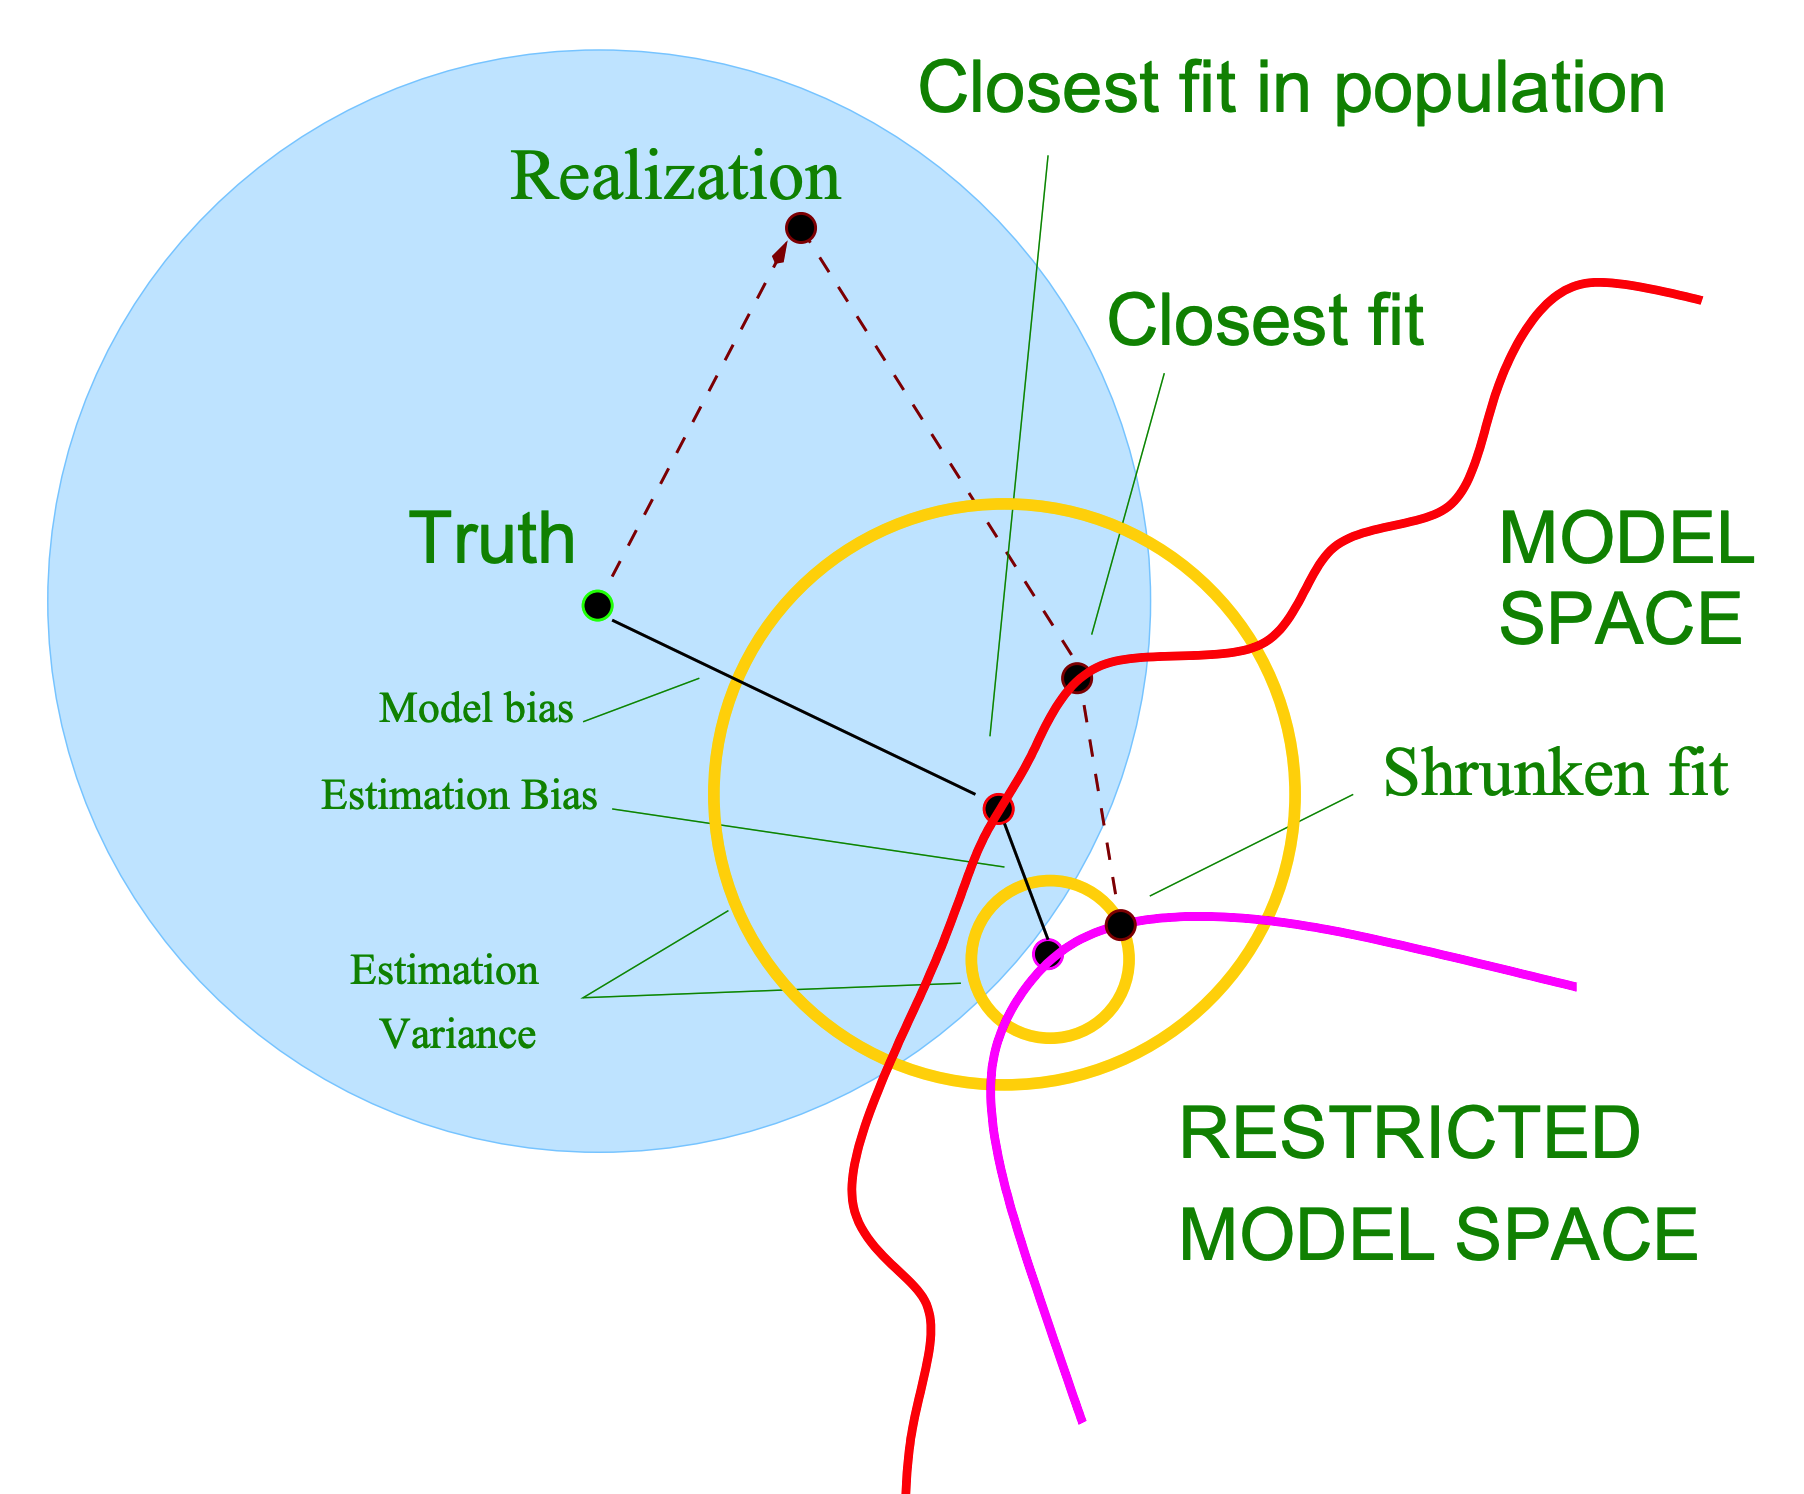
\includegraphics[width=0.8\textwidth]{figures/bias_variance}
%\end{figure}
	
	\newpage
	\chapter{Linear Models}
	\begin{tcolorbox}
\begin{tabular}{ll}
	$\bfX \in \R^{n \times d}$ & data matrix\\
	$\bfy \in \R^{n}$ & label vector\\
	$\mathcal{D} = \{(\mathbf{x}_i, y_i) \}_{i=1}^n$ & a data set with samples and labels \\
	$\beta \in \R^d $ & weights \\
	$\lambda \in \R_+$ & regularization scaler \\
\end{tabular}
\end{tcolorbox}

\section{Linear Regression}
\begin{definition}[Linear Regression or OLS]
Let $ y = f(\bfx) = \beta^\top \bfx $ be the target function.
\marginnote{\footnotesize For the bias term, using this trick: $x' = [x_1, x_2, \cdots, x_n, 1]$}[0cm]
The optimization objective of linear regression is 
\begin{equation}
	\min_{\beta}\quad \sum_{i=1}^n (y_i - \beta^\top \bfx_i)^2
\end{equation}
\end{definition}
Here, the objective is to obtain the minimal squared error, so it is also called ``Ordinary Least Squared'' (OLS) method.

Instead of the squared error, other loss functions might also be used here. For example, with the the $L_p$ distance, we have
\begin{equation}
	\min_{\beta}\quad \sum_{i=1}^n \norm{ y_i - \beta^\top \bfx_i}_p
\end{equation}
\marginpar{\footnotesize Derivative of $L_p$:
$\partial \norm{\vec{w}}_p^p / \partial w_j
= p |w_j|^{p-1} \sign(w_j) $
}where $\norm{\bfx}_p = \sqrt[p]{\sum_{i=1}^d{|x_i|^p}} $.
$L_p$ loss is convex when $p \geq 1$.
The $L_1$ loss puts less emphasis on large outliers.
For a large $p$, the results are restricted to a region.
For $0 \leq p < 1$, the function becomes non-convex but is even more
robust towards outliers.

\subsection{Ridge Regression}
\begin{definition}[Ridge Regression]
To condition the model's complexity, it is common to use the method called ``Ridge regression'', which introduces a $L_2$ constraint on the weight. 
\begin{equation}
	\min_{\beta}\quad \left\{\sum_{i=1}^{n}\left(y_{i}-\beta^{\top} \mathbf{x}_{i}\right)^{2} \right\}, \quad s.t.\ \sum_{j=1}^{d}\beta_{j}^2 \leq t.
\end{equation}
\end{definition}
Using  Lagrange multipliers, it can be re-written into, 
\marginpar{\footnotesize Should be $\lambda(\sum_j \beta^2_j - t)$, but $-\lambda t$ can be omitted since it is a constant.}
\begin{equation}
\widehat{\beta}=\argmin _{\beta}\ \left\{\sum_{i=1}^{n}\left(y_{i}-\beta^{\top} \mathbf{x}_{i}\right)^{2}+\lambda \sum_{j=1}^{d}\beta_{j}^2 \right\} 
\end{equation}
Note that, here $\lambda$ and $t$ has a one-to-one relationship.
$L_2$ regression on weights is also called the ``weight decay'', as it decays weights to zero.

\begin{property}
Ridge regression has a \textbf{closed-form} solution of
\begin{equation}
\widehat{\beta} = (\bfX ^\top \bfX + \lambda \bfI )^{-1} \bfX^\top \bfy.
\end{equation}
\end{property}
\begin{proof} Let
\begin{align}
	\widehat{\beta} & = \argmin_\beta\ J(\beta; \bfX, \bfy) :=  \argmin_\beta\ (\bfy-\beta^\top \bfX)^\top(\bfy-\beta^\top \bfX)+\lambda \beta^\top \beta
\end{align}
The derivative of $J(\beta; \bfX, \bfy)$ is 
\begin{align}
	\widehat{\beta} & = \argmin_\beta\ (\bfy-\beta^\top \bfX)^\top(\bfy-\beta^\top \bfX)+\lambda \beta^\top \beta
\end{align}
%\textit{Proof.} The objective can be written as,
%\begin{equation}
%	\begin{aligned}
%		\min_{\beta}\ \sum_i (y_i - \beta^\top \bfx_i)^2 + \lambda || \beta ||_2^2 & = \min_{\beta}\ (\bfy - \beta^\top \bfx)^\top (\bfy - \beta^\top \bfx) + \lambda  \beta^\top \beta \\
% 	& =\min_{\beta}\ (\bfy^\top \bfy - \bfx^\top \beta \bfy - \bfy^\top \beta^\top \bfx + \bfx^\top \beta \beta^\top \bfx) + \lambda  \beta^\top \beta \\
%		& \doteq J(\beta)
%	\end{aligned}
%\end{equation}
By differentiating the above equation and equating it to zero, we can get the optimal point.
\begin{equation}
\begin{aligned}
	0 & = \frac{\partial J(\beta)}{\partial \beta} \\
	& = -2 \bfX^\top \bfY + 2 \bfX^\top \bfX \beta + 2 \lambda \beta \\
\end{aligned}
\end{equation} 
Therefore,
\begin{equation}
	(\bfX^\top \bfX + \lambda \bfI) \beta = \bfX^\top \bfY
\end{equation}
Multiplying $(\bfx^\top \bfx + \lambda \bfI)^{-1}$ on both sides, we get
\begin{equation}
	\hat{\beta} = (\bfX^\top \bfX + \lambda \bfI)^{-1} \bfX^\top \bfY
\end{equation}
\end{proof}

Alternatively, the gradient descent can also be used to find the global optimum of ridge regression, since its objective is convex.
The closed-form solution takes $\mathcal{O}(n^3)$ time. The gradient descent solution takes $\mathcal{O}(n d \log (1 / {\epsilon}))$ time.
When $n$ becomes larger, the gradient descent method will be more efficient than closed-form solution.

\subsection{Lasso Regression}
Lasso regression is the linear regression whose weights regularized by $L_1$. The objective then becomes,
\begin{equation*}
\min_{{\beta}}\ \ {
	\sum_{i=1}^n{(y_i - {w}^T {\bfx}_i)^2
		+ \lambda \norm{{\beta}}_1
}}
\end{equation*}
The $L_1$ penalty, in theory, encourages coefficients to be
exactly zero. In ridge regression, weights decay relatively smoothly;
in lasso regression, some weights may heavily increase
with increasing $\lambda$. This results in some form in automatic feature selection. However, there is \textbf{no} closed-form solution for lasso regression.


\section{Bias and Variance Trade-off}
\subsection{From Optimization Perspective}
\paragraph{Expectation of Bias} Ridge regression produces a \textbf{biased estimator} of the true parameter $\beta^*$. 
The expectation of $\widehat{\beta}$ is,
\begin{align}
	\EEE{\widehat{\beta} \mid \bfX} & =  (\bfX ^\top \bfX + \lambda \bfI )^{-1} \bfX^\top \EE [\bfy\mid \bfX] \\
	& = (\bfX ^\top \bfX + \lambda \bfI )^{-1} \bfX^\top \bfX \beta^* \quad \mathrm{(recall\ that } \ \bfy = \bfX \beta^* \mathrm{)} \\
	& = (\bfX ^\top \bfX + \lambda \bfI )^{-1} (\bfX^\top \bfX + \lambda \bfI - \lambda \bfI)\beta^* \\
	& = [\bfI - \lambda (\bfX ^\top \bfX + \lambda \bfI )^{-1}] \beta^*
\end{align}
So, the expectation of bias is,
\begin{equation}
	\EEE{\beta^* - \widehat{\beta} \mid \bfX} = \lambda (\bfX ^\top \bfX + \lambda \bfI )^{-1} \beta^*.
\end{equation}

\paragraph{Bias under Noisy Label}
Let $\bfy = \bfX \beta^* + \xi$, $\xi \sim N(0, \sigma^2 \bfI)$. Conduct SVD decomposing on $\bfX \in \R^{n \times d}$,
\begin{equation}
	\bfX = \bfU \bfD \bfV^\top. \label{eq:svd_x}
\end{equation} 
When $\lambda=0$, the solution of $\widehat{\beta}$ is \marginpar{\footnotesize $ (\bfX ^\top \bfX )^{-1} = \\ (\bfV \bfD^\top \bfU^\top \bfU \bfD \bfV^\top)^{-1}  \\ {=(\bfV \bfD^\top \bfD \bfV^\top)^{-1}} \\ {= (\bfV^\top)^{-1} (\bfD^\top \bfD)^{-1} \bfV^{-1}} \\ {= \bfV (\bfD^\top \bfD)^{-1} \bfV^{-1}}  $. Thus, $ (\bfX ^\top \bfX )^{-1} \bfX^\top = \\ {\bfV (\bfD^\top \bfD)^{-1} \bfV^{-1}}\bfV \bfD^\top \bfU^\top \\ {= \bfV (\bfD^\top \bfD)^{-1} \bfD^\top \bfU^\top } \\ {= \bfV \bfD ^+ \bfU^\top}.$}
\begin{align}
	\widehat{\beta} & = (\bfX ^\top \bfX )^{-1} \bfX^\top \bfy \\
	& = (\bfX ^\top \bfX )^{-1} \bfX^\top (\bfX \beta^* + \xi) \\
	& = \beta^* + (\bfX ^\top \bfX )^{-1} \bfX^\top \xi.
\end{align}
Insert Eq. \ref{eq:svd_x}, we have 
\begin{align}
	\widehat{\beta} - \beta^* & =  (\bfX ^\top \bfX )^{-1} \bfX^\top \xi \\
	& = \bfV \bfD ^+ \bfU^\top \xi.
\end{align} 
Here, $ \bfD ^+ $ is the Moore-Penrose pseudo inverse matrix of $\bfD$.

\subsection{From Bayesian Perspective} \marginpar{\footnotesize Reference: Probabilistic AI, Lecture 2}
\paragraph{Equivalence to Bayes}
Assume the prior distribution of $\beta$ is $p(\beta) = \mathcal{N}(0, \sigma_p^2 \cdot \bfI)$, and it is independent of $\bfx_i$. Also, we assume the labels $y_i$ have some independent Gaussian noise, i.e. $y_i = \beta^\top \bfx_i + \xi_i$, $\xi \sim \mathcal{N}(0, \sigma_n^2)$. Then, the Ridge regression can be viewed as a \textbf{Bayesian inference}, where 
\begin{equation}
	\lambda = \sigma_n^2/\sigma_p^2
\end{equation}
\begin{proof} 
According to the noise assumption, the likelihood of $y_{1:n}$ is
\begin{equation}
\begin{aligned}
		p(y_{1: n} \mid \beta, \bfx_{i: n}) & = \prod_{i=1}^n p(y_i \mid w_1, x_i) = \mathcal{N}(y_i; \beta^\top \bfx, \sigma_n^2)
\end{aligned}
\end{equation}
First, using Bayes' rule, we obtain the posterior of $\beta$,\begin{equation}
\begin{aligned}
	p(\beta \mid \bfx_{1:n}, y_{1:n}) & = \frac{1}{Z} p(\beta \mid \bfx_{1:n}) p(y_{1:n} \mid \beta, \bfx_{1:n}) \marginnote{\footnotesize\textit{This is Bayes' rule $p(\beta\mid y) = p(\beta) p(y \mid \beta) / p(y)$ given $\bfx$}}[0cm]
	\\
	& = \frac{1}{Z} p(\beta) \prod_i p(y_i \mid \beta, \bfx_i) \\
	& = \frac{1}{Z} \frac{1}{Z_p} \exp\left( -\frac{1}{2 \sigma_p^2} || \beta ||^2\right) \cdot \frac{1}{Z_l} \prod_i \exp\left( -\frac{1}{\sigma_n^2} (y_i - \beta^\top \bfx_i)^2 \right) \\
	& = \frac{1}{Z Z_p Z_l} \exp\left( -\frac{1}{2 \sigma_p^2} || \beta ||^2 - \frac{1}{2\sigma_n^2}\sum_{i=1}^n (y_i - \beta^\top \bfx_i)^2 \right)
	\end{aligned}
\end{equation}
Here, $Z$, $Z_p$, $Z_l$ are the normalizers: $Z = p(y_{1:n} \mid \bfx_{1:n})$, $Z_p = \sqrt{2\pi} \sigma_p$, $Z_l = (2\pi)^{(n/2)} \sigma_n $. 

Next, we maximize the posterior of $\beta$,
\begin{equation}
	\argmax_{\beta}\ p(\beta \mid \bfx_{1:n}, y_{1:n}) = \argmax_{\beta}\ \underbrace{\sum_{i=1}^n (y_i - \beta^\top \bfx_i)^2}_\mathrm{OLS} + \underbrace{\frac{\sigma_n^2}{\sigma_p^2} \norm{\beta}^2}_{\lambda \cdot  L_2\mathrm{Reg.}}
\end{equation} 
Note that the posterior has the same form of the Ridge Regression when $\lambda$ has the value of $\sigma_n^2 / \sigma_p^2$.  Hence, the Ridge Regression (Eq.~\ref{eq:rr}) can be viewed as a Bayesian Inference process theoretically.
\end{proof}

\paragraph{Uncertainty}
	From a Bayesian perspective, we can not only know the optimal solution, we can also obtain the uncertainty for such solution. The uncertainty is denoted by variance of the posterior $p(\beta \mid \bfx_{1:n}, y_{1:n}) = \mathcal{N}(\bar{\mu}, \bar{\Sigma})$. The mean and variance of the posterior are,
\begin{equation}
\begin{array}{l}
\bar{\mu}=\left(\bfx^{\top} \bfx+\sigma_{n}^{2} \bfI\right)^{-1} \bfx^{\top} \bfy \\
\bar{\Sigma}=\left(\sigma_{n}^{-2} \bfx^\top \bfx+\bfI\right)^{-1}
\end{array}
\end{equation}
\begin{proof} 
We can get the close-form of the posterior.\footnote{For more details, please check here \url{https://en.wikipedia.org/wiki/Bayesian_linear_regression}}.
\marginpar{\footnotesize ${\bfu^\top \bfA \bfu - 2\alpha^\top \bfu} = {(\bfu - \bfA^{-1}\alpha)^\top \bfA} (\bfu - \bfA^{-1}\alpha)$}
\begin{equation}
	\begin{aligned}
		p(\beta\mid \bfx_{1:n}, y_{1:n}) & = \frac{1}{Z Z_p Z_l} \exp \left( -\frac{1}{2\sigma_p^2} || \beta ||^2 -\frac{1}{2\sigma_n^2} \sum_i || y_{i} - \beta^\top \bfx_{i} ||^2 \right) \\
		& = \frac{1}{Z Z_p Z_l} \exp \left( -\frac{1}{2\sigma_p^2}\beta^\top \beta -\frac{1}{2\sigma_n^2}(\bfy^\top \bfy\ - 2 \bfy \beta^\top \bfx + \beta^\top \bfx^\top \bfx \beta) \right) \\
		& \propto \exp \left( -\frac{1}{2} \left( \beta^\top (\frac{1}{\sigma_n^2} \bfx^\top \bfx + \frac{1}{\sigma_p^2} \bfI ) \beta -2(\bfx^\top \bfy)^\top \beta \right) \right) \\
		& = \exp \left( -\frac{1}{2}(\beta - {{\mu}}')^\top {{\Sigma}}'^{-1} (\beta - {{\mu}}') \right)
	\end{aligned}
\end{equation}
Here, 
\begin{equation}
	\begin{aligned}
		{{\mu}}' & = (\sigma_n^{-2} \bfx^\top \bfx + \sigma_p^{-2} \bfI )^{-1} \bfx^\top \bfy \\
		{{\Sigma}}' & = (\sigma_n^{-2} \bfx^\top \bfx + \sigma_p^{-2}\bfI )^{-1}
	\end{aligned}
\end{equation}
After normalization, we can get the answer
\begin{equation}
\begin{array}{l}
\bar{{\mu}}=\left(\bfx^{\top} \bfx+\sigma_{n}^{2} \bfI\right)^{-1} \bfx^{\top} \bfy \\
\bar{{\Sigma}}=\left(\sigma_{n}^{-2} \bfx^\top \bfx+\bfI\right)^{-1}
\end{array}
\end{equation}
\end{proof}

\paragraph{Uncertainty in Prediction}
	Define $f^* = \beta^\top \bfx^*$ as the model's output at $\bfx^*$. The uncertainty of the prediction is $$\bfx^{*\top}{\bar\Sigma} \bfx^* + \sigma_n^2.$$
\begin{proof}
\begin{equation}
	p(f^* \mid \bfx_{1:n}, y_{1:n}, \bfx^*) = \int p(f^*\mid \beta, \bfx^*)\ p(\beta \mid \bfx_{1:n}, y_{1:n}, \bfx^*) \mathrm{d} \beta
\end{equation}
Since $\beta \sim \mathcal{N}(\bar{\mu}, \bar{\Sigma})$,
\begin{equation}
	p(f^* \mid \bfx_{1:n}, y_{1:n}, \bfx^*) = \mathcal{N}({\bar\mu}^\top \bfx^*, \bfx^{*\top}{\bar\Sigma} \bfx^*)
\end{equation}
Since $y^* = f^* + \xi$, $\xi \sim \mathcal{N}(0, \sigma_n^2)$,
\begin{equation}
	p(y^* \mid \bfx_{1:n}, y_{1:n}, \bfx^*) = \mathcal{N}({\bar\mu}^\top \bfx^*, \bfx^{*\top}{\bar\Sigma} \bfx^* + \sigma_n^2)
\end{equation}
Here, $\bar{{\mu}}$ and $\bar{{\Sigma}}$ are the mean and variance of posterior, respectively.
\end{proof}

Moreover, we can distinguish two forms of uncertainty:
\begin{enumerate}
	\item \textbf{Epistemic uncertainty} ($\bfx^{*\top}{\bar\Sigma} \bfx^*$): Uncertainty about the model due to the lack of data.
	\item \textbf{Aleatoric uncertainty} ($\sigma_n^2$): Irreducible noise from measurement.
\end{enumerate}

\section{Linear Discriminative Analysis (LDA)}
\subsection{Fisher's Linear Discriminant}
To separate two classes of data points, Fisher's idea is to find a hyper-plane, on which the data points project with  maximal distance between the centers and minimal variance within the class.
\begin{definition}[Separation]
	Suppose two classes of observations have mean $\bfmu_1, \bfmu_2$ and covariances $\Sigma_1, \Sigma_2$. The separation between these two distributions is
	$$
	S(\bfw) =\frac {\sigma_{\text{between}}^{2}}{\sigma _{\text{within}}^{2}}={\frac {({ {\bfw}}\cdot { {\bfmu }}_{1}-{ {\bfw}}\cdot { {\bfmu }}_{2})^{2}}{{ {\bfw}}^\top\Sigma _{1}{ {\bfw}}+{ {\bfw}}^\top\Sigma _{2}{ {\bfw}}}}={\frac {({ {\bfw}}^\top ({ {\bfmu }}_{1}-{ {\bfmu }}_{2}))^{2}}{{ {\bfw}}^\top(\Sigma _{1}+\Sigma _{2}){ {\bfw}}}} := \frac{\bfw^\top \mathbf{S}_b \bfw}{\bfw^\top \mathbf{S}_w \bfw}
	$$
	Here, $\mathbf{S}_b = (\bfmu_1-\bfmu_2) (\bfmu_1-\bfmu_2)^\top $ and $\mathbf{S}_w = \Sigma _{1}+\Sigma _{2}$.
\end{definition}
\begin{theorem}[Solution]
	The optimal solution of $\max_\bfw S(\bfw)$ satisfies
	$$
	\bfw^* \propto \mathbf{S}_{w}^{-1}(\bfmu_1 - \bfmu_2).
	$$
\end{theorem}
\begin{proof}
	Setting the derivatives of $S$ to $0$, we have
	\begin{align}
		0 = \diff{\bfw}S(\bfw) & = \frac{\bfw^\top \mathbf{S}_w \bfw \cdot 2\mathbf{S}_b \bfw - \bfw^\top \mathbf{S}_b \bfw \cdot 2\mathbf{S}_w \bfw}{(\bfw^\top \mathbf{S}_w \bfw)^2}  \\
		\Longrightarrow \quad &  \bfw^\top \mathbf{S}_w \bfw \cdot \mathbf{S}_b \bfw - \bfw^\top \mathbf{S}_b \bfw \cdot \mathbf{S}_w \bfw = 0 \\
		\Longrightarrow \quad &   \mathbf{S}_w^{-1} \mathbf{S}_b \bfw =\frac{ \bfw^\top \mathbf{S}_b \bfw}{\bfw^\top \mathbf{S}_w \bfw} \cdot  \bfw \\		
		\Longrightarrow \quad &   \mathbf{S}_w^{-1} \mathbf{S}_b \bfw = \lambda  \bfw, \where \lambda = \frac{ \bfw^\top \mathbf{S}_b \bfw}{\bfw^\top \mathbf{S}_w \bfw}. \\	
	\end{align}
	This is an eigenvalue problem. However, consider the fact that $\mathbf{S}_b \bfw = (\bfmu_1-\bfmu_2) (\bfmu_1-\bfmu_2)^\top \bfw $, we have
	\begin{equation}
		\mathbf{S}_w^{-1} \mathbf{S}_b \bfw = \mathbf{S}_w^{-1} [\beta (\bfmu_1-\bfmu_2)] = \beta [\mathbf{S}_w^{-1} (\bfmu_1-\bfmu_2)], \where \beta = (\bfmu_1-\bfmu_2)^\top \bfw,
	\end{equation}
	which means the solution of the eigenvalue problem is just $\bfw^* = \beta \mathbf{S}_w^{-1} (\bfmu_1-\bfmu_2)$.
\end{proof}
\subsection{LDA with Gaussian Prior}
\begin{definition}
	One way to employ linear model to classification problem is Linear Discriminative Analysis (LDA). It given the probability of a sample $\bfx$ lying in the positive class,
	\begin{equation}
		p(y = 1 \mid \bfx) = \sigma(w^\top \bfx + w_0), \where \sigma(\bfx) = \frac{1}{1 + \exp(-\bfx)}
	\end{equation}
\end{definition}
\begin{proof}
	\begin{align}
		p(y = 1\mid \bfx) & = \frac{p(\bfx \mid y = 1)\, p(y = 1)}{p(\bfx \mid y = 1)\, p(y = 1) + p(\bfx \mid y = 0)\, p(y = 0)} \\
		& = \frac{1}{1 + \frac{p(\bfx \mid y = 0)\, p(y = 0)}{p(\bfx \mid y = 1)\, p(y = 1)}}\\
		& = \frac{1}{1 + \exp\left(-\log  \frac{p(\bfx \mid y = 1)\, p(y = 1)}{p(\bfx \mid y = 0)\, p(y = 0)}\right) }\label{eq:lda1}
	\end{align}
If we assume that all $p(\bfx \mid y=i)$ are Gaussian distributions with the same variance $\Sigma$, we have
\begin{equation}
	\log p(\bfx \mid y=i) = -\frac{1}{2} \log |2 \pi \Sigma| - \frac{1}{2} \bfx^\top \Sigma^{-1} \bfx + \bfx^\top \Sigma^{-1} \mu_i - \frac{1}{2} \mu_i^\top \Sigma^{-1} \mu_i
\end{equation}
Then, \marginpar{\footnotesize ${w^\top \bfx = \bfx^\top w \in \R}$}
\begin{equation}
	\log \frac{p(\bfx \mid y = 1)\, p(y = 1)}{p(\bfx \mid y = 0)\, p(y = 0)} = \underbrace{\bfx^\top \Sigma^{-1}(\mu_1 - \mu_0)}_{\mathbf{x}^\top w} \underbrace{- \frac{1}{2}(\mu_1 \Sigma^{-1} \mu_1 - \mu_0 \Sigma^{-1} \mu_0) + \log \frac{p(y=1)}{p(y=0)}}_{w_0} \label{eq:lda}
\end{equation}
Insert Eq.~\ref{eq:lda} to Eq.~\ref{eq:lda1}, we have
\begin{equation}
	p(y = 1\mid \bfx) = \frac{1}{1 + \exp(w^\top \bfx + w_0)}
\end{equation}
This proof provides some intuition of the \textit{sigmoid} function $\sigma$. 
\end{proof}

\subsection{Quadratic Discriminative Analysis}
\begin{definition}
	We can extend LDA by using a quadratic function, named Quadratic Discriminative Analysis (QDA). It can model the clusters with different variance. It given the probability of a sample $\bfx$ lying in the positive class as,
	\begin{equation}
		p(y = 1 \mid \bfx) = \sigma(\bfx^\top W \bfx + w^\top \bfx + w_0), \quad \text{where}\ \sigma(\bfx) = \frac{1}{1 + \exp(-\bfx)}
	\end{equation}
\end{definition}
\begin{proof}
	Similar to LDA, but $p(\bfx \mid y=i)$ are Gaussian distributions with different variance of $\Sigma_i$.
\end{proof}
	
	\newpage
	\chapter{Support Vector Machine}
	\section{Lagrange Duality \& KKT Conditions}
Considering the following optimization problem for $\bfx \in \R^d$ with constraints $g(\bfx) \leq 0$ and $h(\bfx) = 0$, 
\begin{equation}
	\min_\bfx\ f(\bfx), \quad s.t.\ g_i(\bfx) \leq 0, h_j(\bfx) = 0 \quad (\forall i=[m], j=[n]),
\end{equation}
One can form the \textbf{generalized Lagrangian} as
\begin{equation}
	\cL(\bfx, \mu, \lambda) = f(\bfx) + \sum_i \mu_i g_i(\bfx) + \sum_j \lambda_j h_j(\bfx), \quad \mu_i \geq 0.
\end{equation}
Here, $\mu_i$ and $\lambda_j\ (i=[m], j=[n])$ are the Lagrange multipliers.

\subsection{Primal and Dual Problem}
With the generalized Lagrangian, the original problem can be turned into an optimization problem without constraints. There are two ways for doing so, which pose the ``primal'' and ``dual'' problem, respectively. 
\begin{figure}[h]
\centering
\begin{tikzpicture}
\tikzstyle{block} = [minimum size=1.5cm,draw,text width=5cm,text centered]
\draw (0,0.5) node[block,minimum size=1.75cm,label=above:original problem] (a) {
$\begin{aligned}
	\min_\bfx & \quad f(\bfx), \\ s.t. & \quad g_i(\bfx) \leq 0, h_j(\bfx) = 0 
\end{aligned}$};
\draw (-5,-2) node[block,label=above:primal problem] (b) {
$\begin{aligned}
	\theta_p(\bfx) = \max_{\mu \geq 0, \lambda}\ \cL(\bfx, \mu, \lambda)
\end{aligned}$};
\draw (5,-2) node[block,label=above:dual problem] (c) {
$\begin{aligned}
	\theta_d(\mu, \lambda) = \min_{\bfx}\ \cL(\bfx, \mu, \lambda)
\end{aligned}$};
\draw (-5,-4.5) node[block,label=below:minimize the primal problem] (d) {
$\begin{aligned}
	p^* = \min_{\bfx}\max_{\mu \geq 0, \lambda}\ \cL(\bfx, \mu, \lambda)
\end{aligned}$};
\draw (5,-4.5) node[block,label=below:maximize the dual problem] (e) {
$\begin{aligned}
	d^* = \max_{\mu \geq 0, \lambda} \min_{\bfx}\ \cL(\bfx, \mu, \lambda)
\end{aligned}$};
\draw (0,-4.5) node[minimum size=1.2cm,draw,text centered,text width=2.75cm] (f) { \footnotesize
$p^* \geq d^*$ 
$\textbf{KKT} \Longrightarrow p^* = d^*$
};
\draw[->] (a) -- (b);
\draw[->] (a) -- (c);
\draw[->] (b) -- (d);
\draw[->] (c) -- (e);
\draw[dashed] (e) -- (f);
\draw[dashed] (d) -- (f);
\end{tikzpicture}
\end{figure}

The primal problem and dual problem have the same objective, except that the order of the ``max'' and the ``min'' are exchanged.

\subsection{KKT Conditions}
The Karush-Kuhn-Tucker (KKT) theorem state a \textbf{necessary condition} that there must exist $(\bfx^*, \mu^*, \lambda^*)$ that is the solution for both primal problem and dual problem, and moreover $p^* = d^* = \cL(\bfx^*, \mu^*, \lambda^*)$. The KKT conditions are as follows,
\begin{align}
	\diff{x_i} \cL(\bfx^*, \mu^*, \lambda^*) &= 0, \quad i = [d] \\
	\diff{\lambda_j} \cL(\bfx^*, \mu^*, \lambda^*) &= 0, \quad j = [n] \\
	\mu^*_i g_i(\bfx^*) &= 0, \quad i = [m] \qquad (\text{``dual complementarity''}) \\
	 g_i(\bfx^*) & \leq 0, \quad i = [m] \\
	 \mu_i^* &\geq 0, \quad i = [m]
\end{align}

\section{Original SVM}
\subsection{Hard-margin SVM}
\begin{definition}[SVM - Primal Problem]
Given a training dataset of $n$ points of the form $(\bfx_i, y_i), \ y_i = \{1, -1\}$, the SVM algorithm finds the optimal hyper-plan $\bfw^\top \bfx + w_0 = 0$ that separates the positive and negative points with the maximum margin. More formally,
\begin{align}
	\min_{\bfw, w_0} & \quad \onehalf \norm{\bfw}^2  \\
	s.t. & \quad y_i (\bfw^\top \bfx_i + w_0) \geq 1, \quad i = [n]
\end{align}
\end{definition}
\begin{definition}[SVM - Dual Problem]
The Lagrangian dual problem of SVM is given by
\begin{align}
	\max_{\alpha} & \quad \sum_{i} \alpha_i - \onehalf \sum_{i,j} \alpha_i \alpha_j y_i y_j \langle \bfx_i, \bfx_j \rangle  \\
	s.t. & \quad \alpha_i \geq 0,\ \sum_{i} \alpha_i y_i = 0
\end{align}
\end{definition}
\begin{proof}
	We show that how SVM's primal problem can be turned into its dual problem. We first construct the Lagrangian
	\begin{equation}
		\cL(\bfw, w_0; \alpha) = \onehalf \norm{\bfw}^2 - \sum_{i \leq n} \alpha_i [y_i(\bfw^\top \bfx + w_0) - 1].\label{eq:svm_lag}
	\end{equation}
	To get the dual problem $\theta_d(\alpha)$, we need to minimize the Lagrangian by setting its derivatives to $0$,
	\begin{align}
		\mathbf{0} = \nabla_\bfw \cL(\bfw, w_0; \alpha) = \bfw - \sum_{i \leq n} \alpha_i y_i \bfx_i \quad & \Longrightarrow\quad \bfw^* = \sum_{i \leq n} \alpha_i y_i \bfx_i, \\
		{0} = \diff{w_0} \cL(\bfw, w_0; \alpha) = \sum_{i \leq n} \alpha_i y_i \quad & \Longrightarrow\quad  \sum_{i \leq n} \alpha_i y_i = 0.	
	\end{align}
	If we plug them back into Eg.~\ref{eq:svm_lag}, we have
	\begin{equation}
		\cL(\bfw^*, w_0^*; \alpha) = \sum_{i \leq n} \alpha_i - \onehalf \sum_{i, j} \alpha_i \alpha_j y_i y_j \bfx_i^\top \bfx_j - \underbrace{w_0 \sum_{i \leq n} \alpha_i y_i}_{=0},
	\end{equation}
	Then the dual problem is achieved as
	\begin{align}
	\max_{\alpha} & \quad \cL(\bfw^*, w_0^*; \alpha) = \sum_{i} \alpha_i - \onehalf \sum_{i,j} \alpha_i \alpha_j y_i y_j \langle \bfx_i, \bfx_j \rangle  \\
	s.t. & \quad \alpha_i \geq 0,\ \sum_{i} \alpha_i y_i = 0
\end{align}
\end{proof}

\remark The SVM can be more efficiently calculated in its dual form, because we can easily find the support vectors (whose $\alpha_i = 0$) and then derive the classification results directly by
\begin{equation}
	f(\bfx_*) = \bfw^\top \bfx_* + w_0 = w_0 + \sum_{\{i \mid \alpha_i > 0\}} \alpha_i y_i \langle \bfx_i, \bfx_* \rangle.
\end{equation}
It should be noticed that the hard-margin SVM requires both assumptions to work:
\begin{itemize}
	\item The data points are linearly separable;
	\item There exists a separating hyperplane with non-zero margin.
\end{itemize}

\subsection{Soft-margin SVM}
\begin{definition}[SoftSVM - Primal Problem]
\begin{align}
	\min_{\bfw, w_0} & \quad \onehalf \norm{\bfw}^2 + C \sum_{i \leq n} \xi_i \\
	s.t. & \quad y_i (\bfw^\top \bfx_i + w_0) \geq 1 - \xi_i,\ \ \xi_i > 0
\end{align}
\end{definition}
\begin{definition}[SoftSVM - Dual Problem]
\begin{align}
	\min_{\alpha} & \quad \onehalf \sum_{i} \alpha_i - \onehalf \sum_{i,j} \alpha_i \alpha_j y_i y_j \langle \bfx_i, \bfx_j \rangle \\
	s.t. & \quad 0 \leq \alpha_i \leq C,\ \sum_{i} \alpha_i y_i = 0
\end{align}
\end{definition}
\begin{proof}
	Similar to hard-margin SVM, given $\alpha_i, \beta_i \geq 0$, we have
	\begin{equation}
		\cL(\bfw, w_0, \xi; \alpha) = \onehalf \norm{\bfw}^2 + C \sum_{i \leq n} \xi_i  - \sum_{i \leq n} \alpha_i [y_i(\bfw^\top \bfx + w_0) - 1 + \xi_i] - \sum_{i \leq n} \beta_i \xi_i.\label{eq:svm_lag2}
	\end{equation}
	Set its derivatives of Lagrangian to $0$:
	\begin{align}
		\mathbf{0} = \nabla_\bfw \cL(\bfw, w_0, \xi; \alpha) = \bfw - \sum_i \alpha_i y_i \bfx_i \quad & \Longrightarrow\quad \bfw^* = \sum_i \alpha_i y_i \bfx_i; \\
		{0} = \diff{w_0} \cL(\bfw, w_0, \xi; \alpha) = \sum_i \alpha_i y_i \quad & \Longrightarrow\quad  \sum_i \alpha_i y_i = 0; \\
		{0} = \diff{\xi_i} \cL(\bfw, w_0, \xi; \alpha) = C - \alpha_i + \beta_i \quad & \Longrightarrow\quad  \alpha_i = C - \beta_i \ \ (i = [n]).	
	\end{align}
	If we plug them back into Eg.~\ref{eq:svm_lag2}, we get
	\begin{equation}
		\cL(\bfw^*, w_0^*; \alpha) = \sum_i \alpha_i - \onehalf \sum_{i, j} \alpha_i \alpha_j y_i y_j \bfx_i^\top \bfx_j - \underbrace{w_0 \sum_i \alpha_i y_i}_{=0}, \where \alpha_i \leq C.
	\end{equation}
	Then we can obtain the dual problem.
\end{proof}

The optimal solution is given by
\begin{align}
	\bfw^* & = \sum_i \alpha_i^* y_i \bfx_i \\
	\xi_i^* & = \max(0, 1 - y_i(\bfw^{* \top}\bfx_i + w_0^*))
\end{align}

\remark Here, $C$ is a trade-off hyper-parameter. Larger $C$ means narrower margin \& few neglected samples. When $C \rightarrow \infty$, then the solution is approaching to the solution from a hard-margin SVM.

\begin{property}[Hinge Loss Form]
The soft-margin SVM can be also achieved via hinge loss $\ell_{hinge}(\cdot\, , \cdot)$ as
$$
\min_{\bfw, w_0}\quad \sum_{i \leq n} \ell_{hinge}(\bfx_i, y_i) + \frac{1}{2C} \norm{\bfw}^2, \where \ell_{hinge}(\bfx_i, y_i) = \max\left\{0, 1 - y_i (\bfw^\top \bfx_i + w_0 ) \right\}
$$
\end{property}
\remark Since hinge loss is convex and its derivative is known, we can solve the soft-margin SVM directly by gradient descent methods. Note that there is \textbf{no} such loss for hard-margin SVM, because no misclassifications, by definition, will occur in hard-margin SVM.


\section{Extended SVM}

\subsection{Multi-Class SVM}
SVMs can be generalized to a multi-class scenario. The key idea is to maintain $c$ weight vectors $w^{(i)}$, one for each class.
The prediction result is then
\begin{equation}
\hat{y} = \argmax_i \ \ {{w}^{(i) \top} {\bfx}}
\end{equation}
For each data point, it should hold that the prediction
for the true class is separated by a margin from the
class which has the second highest prediction, i.e.
\begin{equation}
w^{(y) \top} \bfx \geq
\max_{i \neq y} \ \ {w^{(i) \top}\bfx} + 1
\end{equation}
Thus, the multi-class Hinge loss is given as
\begin{equation*}
\ell_{hinge}({w}^{(1)}, \cdots, {w}^{(c)}; {\bfx}, y)
= \max{\{0, 1 +
	\max_{j \neq y}\ 
	{{w}^{(j) \top}{\bfx} - {w}^{(y) \top}{\bfx}}
	\}}
\end{equation*}


\subsection{Structured SVM}
Structured SVM generalizes the SVM, which maximizes the margin between the score of the correct class and the score of the highest-scoring incorrect runner-up class (a.k.a. the hard nagetives). 

\begin{definition}[StructuredSVM - Primal Problem]
\begin{align}
	\min_{w, w_0, \xi} & \quad \onehalf \norm{\bfw}^2 + \frac{C}{n} \sum_{1 \leq i \leq n} \xi_i \\
	s.t. & \quad \bfw^\top \Psi(\bfx_i, y_i) - \bfw^\top \Psi(x_i, y) \geq \Delta(y_i, y) - \xi_i,\quad  \xi_i > 0, \quad \forall i\leq n, y \neq y_i,
\end{align}\marginpar{\footnotesize Replacing the margin $1$ with a general function $\Delta(y, y')$.}
where $\Psi: \cX \times \cY \rightarrow \R^{d_1} \times \mathbb{Z}^{d - d_1}$ is a joint-feature map function. $\Delta(\cdot\, , \cdot): \cY \times \cY \rightarrow \R_+$ is function measuring the distance between two labels, which satisfies $\Delta(y, y) = 0$. $\Delta(\cdot\, , \cdot)$ defines the margin of each pair of samples.
\end{definition}


\begin{definition}[StructuredSVM - Dual Problem]
To simplify the notation, let $\Psi_i(y):=\Psi(y_i, \bfx_i)-\Psi(y, \bfx_i)$ and $\Delta_i(y):=\Delta(y, y_i)$. Then, the dual problem is
\begin{align}
	\min_{\alpha} & \quad -\frac{1}{2}\norm{\sum_{i=1}^{n} \sum_{y_{j} \in \mathbb{K}_{i}} \alpha_{i j} \Psi_{i}\left(y_{j}\right)}^{2}+\sum_{i=1}^{n} \sum_{y_{j} \in {K}_{i}} \alpha_{i j} \Delta_{i}\left(y_{j}\right) \\
	s.t. & \quad  0 \leq \sum_{y_{j} \in \mathbb{K}_{i}} \alpha_{i j} \leq C, \quad  \alpha_{i j} \geq 0.
\end{align}
Here, $\mathbb{K}_i = \cY \slash \{y_i\}$.
\end{definition}
\begin{proof}\marginpar{\footnotesize This is taken from the Ex.5-1.}
	Let $\mathbb{K}_i = \cY \slash \{y_i\}$. The Lagrangian is
	\begin{equation}
		\mathcal{L}(\mathbf{w}, \xi, \alpha, \beta)=\frac{1}{2} \mathbf{w}^{\top} \mathbf{w}+C \sum_{i=1}^{n} \xi_{i}-\sum_{i=1}^{n} \sum_{y_{j} \in \mathbb{K}_{i}} \alpha_{i j}\left(\mathbf{w}^{\top} \Psi_{i}\left(y_{j}\right)-\Delta_{i}\left(y_{j}\right)+\xi_{i}\right)-\sum_{i=1}^{n} \beta_{i} \xi_{i}
	\end{equation}
	According to stationary conditions, we have
	\begin{align}
		0 & = \nabla_\bfw \cL = \bfw - \sum_{i = 1}^n  \sum_{y_{j} \in \mathbb{K}_{i}} \alpha_{i j} \Psi_i (y_j), \\
		0 & = \diff{\xi_i} \cL = C - \sum_{y_{j} \in \mathbb{K}_{i}} \alpha_{i j} - \beta_i. \label{eq:ssvm}
	\end{align}
	Plug them into the Lagrangian, we get
	\begin{align}
		\cL(\alpha) = -\frac{1}{2}\norm{\sum_{i=1}^{n} \sum_{y_{j} \in \mathbb{K}_{i}} \alpha_{i j} \Psi_{i}\left(y_{j}\right)}^{2}+\sum_{i=1}^{n} \sum_{y_{j} \in \mathbb{K}_{i}} \alpha_{i j} \Delta_{i}\left(y_{j}\right)
	\end{align}
	Note that, Eq.~\ref{eq:ssvm} also implies $\sum_{y_{j} \in \mathbb{K}_{i}} \alpha_{i j} \leq C$. This concludes the proof.
\end{proof}

\noindent \remark In the dual form, constraints are separable in blocks which is favorable for optimization.

\begin{property}[Similarity with CRF]
The structured SVM can be written into the loss form as
$$
	\min \onehalf \norm{\bfw}^2 + \frac{C}{n} \sum_{1 \leq i \leq n}\left[ \max_{y \in \cY} \ \Delta(y_i, y) - \bfw^\top \Psi(\bfx_i, y_i) + \bfw^\top \Psi(x_i, y) \right]
$$	
The CRF can be formulated as
$$
	\min \frac{ \norm{\bfw}^2}{2\sigma^2} + \sum_{1 \leq i \leq n}\left[ \log \sum_{y \in \cY} \exp\left( \bfw^\top \Psi(\bfx_i, y_i) + \bfw^\top \Psi(x_i, y) \right) \right]
$$
\end{property}
\remark  They both do regularized risk minimization and $\log \sum_y \exp(\cdot)$ can be interpreted as the \texttt{softmax} function.

\begin{table}[hbtp]
\center
{\setstretch{1.3}
\centering
\caption{Summary of some unstructured and structured models}
\begin{tabular}{l l l}
\toprule
\textbf{Training Criteria} & \textbf{Unstructured} & \textbf{Structured}	\\
\midrule
Max posterior's likelihood & Naive Bayes $p(\bfx \mid y)$ & Hidden Markov Model $p(\bfx \mid \bfy)$ \\
Max conditional likelihood  & Logistic / NN $p(y \mid \bfx)$ & Conditional Random Field $p(\bfy \mid \bfx)$ \\
Max margin & SVM $ \alpha^\top \phi(\bfx)$ & Structured SVM $ \alpha^\top \psi(\bfx, \bfy)$ \\
\bottomrule
\end{tabular}
}\end{table}


\newpage
\chapter{Kernel Tricks}
To handle the linear unseparable data, one common method is to use the ``Kernel Trick'' that maps the data into a new high-dimension space.
%\section{Reproducing Kernel Hilbert Space (RKHS)}

\section{Properties of Kernels}
One of the fundamental mathematical results underlying learning theory with kernels is Mercer's theorem.
\begin{definition}[Gram Matrix]
	Let $\cX$ be a closed subset of $ \R^n\ (n \in \mathbb{N})$ and $S = \{ \bfx_1, \cdots, \bfx_n\} \subset \cX$. For any kernel function $K: \cX \times \cX \rightarrow \R$ and its corresponding feature map function $\phi(\bfx): \cX \rightarrow \cH$, the Gram matrix $\bfK$ on $S$ is defined as
	$$
	\bfK =\left[\begin{array}{ccc}
K\left(\bfx_{1}, \bfx_{1}\right) & \cdots & K\left(\bfx_{1}, \bfx_{n}\right) \\
\vdots & & \vdots \\
K\left(\bfx_{n}, \bfx_{1}\right) & \cdots & K\left(\bfx_{n}, \bfx_{n}\right)
\end{array}\right] = \left[\begin{array}{c}
\phi\left(\bfx_{1}\right) \\
\vdots \\
\phi\left(\bfx_{n}\right)
\end{array}\right] \left[\phi\left(\bfx_{1}\right), \cdots, \phi\left(\bfx_{n}\right)  \right],
	$$
	which must be positive semi-definite.
\end{definition}

\begin{theorem}[Mercer's Theorem]
	Let $\cX$ be a closed subset of $ \R^n\ (n \in \mathbb{N})$, $\mu$ a Borel measure on $\cX$, and $K: \cX \times \cX \rightarrow \R$ a symmetric function, i.e., $K(\bfx, \bfy) = K(\bfy, \bfx)$. 
	
	\emph{1. Continuous version}. For any $f \in L^2(\cX, \mu)$, 
	$$
	\iint f(\bfx) K(\bfx, \bfy) f(\bfy) \dxx \dyy \geq 0 \ \Longleftrightarrow\ K(\bfx, \bfy)\text{ is a kernel function},
	$$	
	
	\emph{2. Discrete version}. For any finite set of points $\{x_1, \cdots, x_N\} \subset \cX$ and $f: \cX \rightarrow \R$,
	$$
	\sum_{i, j \leq N} f(\bfx_i) K(\bfx_i, \bfx_j) f(\bfx_j) \geq 0 \ \Longleftrightarrow\  \bff^\top \bfK \bff \geq 0  \ \Longleftrightarrow\  \bfK \in \mathbf{SP_{+}} \text{ is a kernel matrix},
	$$
	where $\bff = [f(x_1), \cdots, f(x_N)]^\top$ and $\bfK$ is the Gram matrix.
\end{theorem}
\remark To become a kernel, the matrix $\bfK$ must be
\begin{itemize}
	\item square and symmetric;
	\item semi-positive definite (can be judged via Sylvester's criterion).
\end{itemize} 

\begin{property}[Kernel Combinations]
Let $K_1: \mathcal{X} \times \mathcal{X} \to \R$
and $K_2: \mathcal{X} \times \mathcal{X} \to \R$
be two kernel functions,
$c > 0$ be a scalar,
$f: \R \to \R$
be either a polynomial with positive coefficients or the
exponential function and
$\mathcal{V} : \mathcal{Z} \to \mathcal{X}$ be a mapping.
Then, the following combinations are also valid kernels:
\begin{itemize}
	\item $K(\bfx, \bfy) = K_1(\bfx, \bfy) + K_2(\bfx, \bfy)$
	\item $K(\bfx, \bfy) = c \cdot K_1(\bfx, \bfy) \quad (c > 0)$
	\item $K(\bfx, \bfy) = K_1(\bfx, \bfy) \cdot K_2(\bfx, \bfy)$
	\item $K(\bfx, \bfy) = g(K_1(\bfx, \bfy))$ ($g$ is a positive-coef. polynomial  or the exponential function)
	\item $K(\bfz, \bfz') = K_1(\mathcal{V}(\bfz), \mathcal{V}(\bfz'))$
\end{itemize}
\end{property} 
\begin{proof} Here we just prove some of them and only consider the matrix form. 

1. For any $\bff$,
\begin{align}
\bff^\top (\bfK_1 + \bfK_2)  \bff = \bff^\top \bfK_1  \bff + \bff^\top \bfK_2 \bff \geq 0.
%	&\iint f(\bfx) \left(K_1(\bfx, \bfy) + K_2(\bfx, \bfy)\right) f(\bfy) \dxx\dyy \\
%	= & \iint f(\bfx) K_1(\bfx, \bfy) f(\bfy) \dxx\dyy + \iint f(\bfx) K_2(\bfx, \bfy) f(\bfy) \dxx\dyy \geq 0.
\end{align}

2. For any $\bff$,
\begin{align}
\bff^\top (c \bfK_1)  \bff = c \ \bff^\top \bfK_1  \bff \geq 0.
\end{align}

3. Let $K_1(\bfx, \bfy) = \phi_1(\bfx)^\top \phi_1(\bfy), K_2(\bfx, \bfy) = \phi_2(\bfx)^\top \phi_2(\bfy)$,
\begin{align}
	K_1(\bfx, \bfy) K_2(\bfx, \bfy) & = \phi_1(\bfx)^\top \phi_1(\bfx) \phi_2(\bfx)^\top \phi_2(\bfx)\\
	& = \sum_{m = 1}^M \phi_1^{(m)}(\bfx)\phi_1^{(m)}(\bfy) \sum_{n = 1}^N \phi_2^{(n)}(\bfx)\phi_2^{(n)}(\bfy) \\
	& = \sum_{m = 1}^M \sum_{n = 1}^N \phi_1^{(m)}(\bfx)\phi_1^{(m)}(\bfy) \phi_2^{(n)}(\bfx)\phi_2^{(n)}(\bfy) \\
	& = \sum_{k = 1}^{MN} \psi_k(\bfx)^\top \psi_k(\bfy) 
\end{align}
where $\psi_k(\bfx) = \mathrm{vec}(\phi_1(\bfx) \phi_2(\bfx)^\top)_k = \phi_1^{(\ceil{k - 1 / N})}(\bfx) \phi_1^{(k - 1 \% N)}(\bfx)$. \marginpar{\footnotesize here, $\ceil{\cdot}$ is for ceiling and \% is for remainder.}

4. Can be proved using previous three conclusions.
\end{proof}

\begin{exercise}[Ex.4-3: Kernel Function] Assume we are given a probability density function $p(\bfx, h)$, where $\bfx \in  \cX$ and $h \in  \cH$ (finite sets). Consider a kernel $k((\bfx, h), (\bfx', h'))$ defined on pairs $(\bfx, h) \in  \cX \times H$. Prove that following function $k_m: \cX \times \cX \rightarrow \R$ defines a kernel.
$$
k_{m}(\mathbf{x}, \mathbf{y})=\sum_{h \in \mathcal{H}} \sum_{h^{\prime} \in \mathcal{H}} k\left((\mathbf{x}, h),\left(\mathbf{y}, h^{\prime}\right)\right) p(h \mid \mathbf{x}) p\left(h^{\prime} \mid \mathbf{y}\right)
$$
\end{exercise}
\begin{sol}
Let $k((\bfx, h), (\bfx', h')) = \phi(\bfx, h)^\top \phi(\bfx', h')$.
\begin{align}
	k_m(\bfx, \bfy) & = \sum_{h \in \cH} \sum_{h' \in \cH} \phi(\bfx, h)^\top \phi(\bfx', h') p(h \mid \mathbf{x}) p\left(h^{\prime} \mid \mathbf{y}\right) \\
	& = \left[ \sum_{h \in \cH} p(h \mid \mathbf{x}) \phi(\bfx, h) \right]^\top \left[ \sum_{h' \in \cH} p(h' \mid \mathbf{y}) \phi(\bfy, h') \right]
\end{align}
This means $k_m(\bfx, \bfy)$ can be decomposed into $\psi(\bfx)^\top \psi(\bfy)$.
\end{sol}


\section{Useful Kernels}
\subsection{Polynomial Kernel}
\begin{definition}[Poly Kernel] Polynomial kernels of degree $d$ over $\bfx \in \R^N$ are defined as
	$$
	K(\bfx, \bfy) = (c + \bfx \cdot \bfy)^d.
	$$
\end{definition}
A polynomial kernel can represent the inner product of two polynomial mappings $\phi(\bfx), \phi(\bfy): \R^N \rightarrow \R^d$ by
	\marginpar{\footnotesize This mapping function $\phi(\bfx)$ is not unique, and may not be the smallest.}
	\begin{equation}
	\phi(\bfx)^\top \phi(\bfy) := K(\bfx, \bfy) = \sum_{i=0}^{d}{d \choose i} c^{d-i}\left(\mathbf{x} \cdot \mathbf{y}\right)^{i},\end{equation}
where
$$\phi(\bfx) = \left[\sqrt{c^d}, \sqrt{d c^{d - 1}} \bfx, \cdots,  \sqrt{{d \choose i}} \bfx^d \right]^\top, \quad \phi(\bfy) = \left[\sqrt{c^d}, \sqrt{d c^{d - 1}} \bfy, \cdots,  \sqrt{{d \choose i}} \bfy^d \right]^\top
$$

\begin{property}[Dimension of Feature Space]\footnote{See slides here: \url{https://cs.nyu.edu/~mohri/ml/ml10/sol3.pdf}} The smallest dimension of the feature space $\phi(\bfx)$ associated to the polynomial kernel $K(\bfx, \bfy): \R^N \times \R^N \rightarrow \R$ of degree $d$ is
$$
{N + d \choose d}.
$$	
\end{property}
\begin{proof}
The dimension of the feature space $\phi(\bfx)$ is thus the number of such monomials $f(N, d) \in \mathbb{Z}$, that is the number of ways of adding $N$ non-negative integers
to obtain a sum of at most $d$. We have
\begin{equation}
	f(N, d) = \underbrace{f(N - 1, d)}_{N\text{ integers with sum of }d} + \underbrace{f(N, d - 1)}_{N\text{ integers with sum at most }d - 1}
\end{equation}
The result then follows by induction on $N + d$, using initial the conditions $f(1, 0) = f(0, 1) = 1$.
\end{proof}
\subsection{RBF Kernel}
The Radial-basis Function (RBF) kernel, also called the Gaussian kernel or squared exponential kernel,
is a popular kernel that is in the form of a radial basis function.
\begin{definition}[RBF Kernel]
With hyperparameter of scale $h$ and variance $\sigma^2$, the RBF kernel is defined as
$$
	k_{RBF}(\bfx, \bfy) = \sigma^2 \exp\left(-\frac{\norm{\bfx - \bfy}^2}{2 h^2} \right).
$$
\end{definition}
The RBF kernel can project vectors into an infinite dimensional space, i.e. $\phi_{RBF}: \R^d \rightarrow \R^\infty$. Without loss of generality, after assuming $\sigma = 1, h = 1/4$, we have
\begin{equation}
	\exp \left(-\norm{\mathbf{x}-\mathbf{y}}^{2}\right)=\sum_{k=0}^{\infty} \underbrace{\left(\sqrt{\frac{1}{k !}} \exp \left(-\norm{\mathbf{x}}^{2}\right) \phi_{\text {poly }}(\mathbf{x})\right)}_{\text {row } k \text { in } \phi_{\mathrm{RBF}}(\mathbf{x})} \cdot \underbrace{\left(\sqrt{\frac{1}{k !}} \exp \left(-\norm{\mathbf{y}}^{2}\right) \phi_{\text {poly }}\left(\mathbf{y}\right)\right)}_{\text {row } k \text { in } \phi_{\mathrm{RBF}}\left(\mathbf{y}\right)}
\end{equation}
\begin{property}[RBF Kernel is Stationary]
	RBF is a stationary kernel, since 
	\begin{equation}
		k_{RBF}(\bfx, \bfy) = k_{RBF}(\bfx + \Delta, \bfy + \Delta) = g(\bfy - \bfx).
	\end{equation}
\end{property}

\subsection{Periodic Kernel}
\begin{definition}
	$$
	k_{Per}(\bfx, \bfy) = \sigma^{2} \exp \left(-\frac{2 \sin ^{2}\left(\pi\left|\bfx-\bfy \right| / p\right)}{h^{2}}\right)
	$$
	Here, the period $p$ simply determines the distance between repetitions of the peaks, and the $h$ determines the length scale function in the same way as in the RBF kernel.
\end{definition}
\begin{property}[Periodic Kernel is Stationary]
	Periodic is a stationary kernel, since 
	\begin{equation}
		k_{Per}(\bfx, \bfy) = k_{Per}(\bfx + \Delta, \bfy + \Delta) = g(\bfy - \bfx).
	\end{equation}
\end{property}

	
	\newpage
	\chapter{Gaussian Process}
	\section{Properties of Gaussian Distribution}
\begin{definition}[Multivariate Gaussian Distribution]
 We say $\bfx = (x_1,\cdots, x_n)$ has a multivariate Gaussian distribution if and only if every linear combination of its components has a (multivariate) Gaussian distribution. Formally,
$$
\bfx \sim \NN(\bfmu, \bfSigma) \Leftrightarrow A \bfx \sim \NN(A\bfmu, A \bfSigma A^\top), \ \forall A.
$$
\end{definition}

\begin{property}[Marginal Distribution]
	From the definition, any subset of random variables $\bfx' \subset \bfx$ are themselves normally distributed, and the mean and covariance is given by simply ignoring all elements that are not in $\bfx'$.
\end{property}

\begin{property}[Conditional Distribution]
	For a joint Gaussian distribution, if we given the values of some RVs $\bfy$, then the conditional distribution of the remaining RVs $\bfy_*$ is
	$$
	p(\bfy_* \mid \bfy) = \NN(\bfmu + \bfSigma_* \bfSigma_{**}^{-1}(\bfy_* - \bfmu_*), \bfSigma - \bfSigma_* \bfSigma_{**}^{-1}\bfSigma_*^\top ),
	$$
	where
	$$
\left[\begin{array}{c}
\bfy \\
\bfy_*
\end{array}\right] 
\sim \mathcal{N}\left(\left[\begin{array}{c}
\bfmu \\
\bfmu_*
\end{array}\right], \left[\begin{array}{cc}
\bfSigma & \bfSigma_* \\
\bfSigma_*^\top & \bfSigma_{**}
\end{array}\right]\right).
	$$
\end{property}
\begin{proof}
By definition, the conditional distribution for $\bfy_*$ given $\bfy$ is
\begin{align}
	p(\bfy_* \mid \bfy) & = \frac{p(\bfy, \bfy_*)}{p(\bfy)} \\
	& \propto \exp\left(-\frac{1}{2}\left[\bfy - \bfmu, \bfy_* - \bfmu_* \right]
\left[\begin{array}{cc}
\bfSigma & \bfSigma_* \\
\bfSigma_*^\top & \bfSigma_{**}
\end{array}\right]^{-1}
\left[\begin{array}{c}
\bfy - \bfmu \\
\bfy_* - \bfmu_*
\end{array}\right] 
\right)
\end{align}  
To get the inverse of covariance matrix, we need to diagonalize it,
\begin{align}
	\left[\begin{array}{cc}
\bfSigma & \bfSigma_* \\
\bfSigma_*^\top & \bfSigma_{**}
\end{array}\right] =
	\left[\begin{array}{cc}
\bmI & - \bfSigma_* \bfSigma_{**}^{-1} \\
0 & \bmI
\end{array}\right]^{-1}
	\left[\begin{array}{cc}
\bfSigma - \bfSigma_* \bfSigma_{**}^{-1} \bfSigma_*^{\top}  & 0 \\
0 & \bfSigma_{**}
\end{array}\right]
	\left[\begin{array}{cc}
\bmI & 0 \\
-\bfSigma_{**}^{-1}\bfSigma_*^\top & \bmI
\end{array}\right]^{-1}
\end{align}
Then, we get the inverse of the covariance matrix,
\begin{align}
	\left[\begin{array}{cc}
\bfSigma & \bfSigma_* \\
\bfSigma_*^\top & \bfSigma_{**}
\end{array}\right]^{-1} =
	\left[\begin{array}{cc}
\bmI & 0 \\
-\bfSigma_{**}^{-1}\bfSigma_*^\top & \bmI
\end{array}\right]
	\left[\begin{array}{cc}
(\bfSigma - \bfSigma_* \bfSigma_{**}^{-1} \bfSigma_*^{\top})^{-1}  & 0 \\
0 & \bfSigma_{**}^{-1}
\end{array}\right]
	\left[\begin{array}{cc}
\bmI & - \bfSigma_* \bfSigma_{**}^{-1} \\
0 & \bmI
\end{array}\right]
\end{align}
Plug it back into the conditional distribution, we get \marginpar{\footnotesize This can be viewed as the product of two Gaussians.}
\begin{align} &\left[\bfy - \bfmu, \bfy_* - \bfmu_* \right]
\left[\begin{array}{cc}
\bfSigma & \bfSigma_* \\
\bfSigma_*^\top & \bfSigma_{**}
\end{array}\right]^{-1}
\left[\begin{array}{c}
\bfy - \bfmu \\
\bfy_* - \bfmu_*
\end{array}\right] \\
=&\left(\bfy-\boldsymbol{\mu}_{1}-\bfSigma_{*}\bfSigma_{**}^{-1}\left(\bfy_*-\boldsymbol{\mu}_{2}\right)\right)^{\mathrm{T}}\left(\bfSigma_{11}-\bfSigma_{*}\bfSigma_{**}^{-1}\bfSigma_{21}\right)^{-1}\left(\bfy-\boldsymbol{\mu}_{1}-\bfSigma_{*}\bfSigma_{**}^{-1}\left(\bfy_*-\boldsymbol{\mu}_{2}\right)\right) \\
& +\left(\bfy_*-\boldsymbol{\mu}_{2}\right)^{\mathrm{T}}\bfSigma_{**}^{-1}\left(\bfy_*-\boldsymbol{\mu}_{2}\right)
\end{align} 
Therefore, the conditional distribution is 
\begin{equation}
	p(\bfy_* \mid \bfy) = \NN(\bfmu + \bfSigma_* \bfSigma_{**}^{-1}(\bfy_* - \bfmu_*), \bfSigma - \bfSigma_* \bfSigma_{**}^{-1}\bfSigma_*^\top )
\end{equation}
\end{proof}

\subsection{Prediction using Gaussian Processes}
\begin{definition}[Gaussian Process]
	A Gaussian Process (GP) is a (potentially infinite) collection of random variables (RV) such that the joint distribution of every finite subset of RVs is multivariate Gaussian:
	$$
	f \sim \mathrm{GP}(\mu(\bfx), K(\bfx, \bfx'))
	$$
where $\mu(\bfx): \cX \rightarrow \cX$ and $K(\bfx,\bfx'): \cX \times \cX \rightarrow \R $ are the mean and covariance function, respectively.
\end{definition}
Now, in order to model the predictive distribution $P(\bff_*\mid \bfx_*, D)$ we can use a Bayesian approach by using a GP prior: $p(\bff \mid \bfx)\sim \mathcal{N}(\mu, \bfSigma)$ and condition it on the training data $D$ to model the joint distribution of $\bff=f(\bfx)$ (vector of training observations) and $\bff_*=f(\bfx_*)$ (prediction at test input).


\begin{definition}[Predictive Distribution under Noise]
Let $y_i = f_i + \epsilon_i$, where $\EE[y_i] = 0$ and $\epsilon_i \sim \NN(0, \sigma^2)$. The predictive density $p(y_{n + 1} \mid \bfx_{n + 1}, \bfX, \bfy)$ for a new data point $\bfx_{n + 1}$ can be obtained analytically in Gaussian Process by deriving the joint distribution
$$
	p\left(\left[\begin{array}{c}
\mathbf{y} \\
y_{n+1}
\end{array}\right] \bigg|\ \bfx_{n+1}, \mathbf{X}, \sigma\right)=\mathcal{N}\left(\left[\begin{array}{c}
\mathbf{y} \\
y_{n+1}
\end{array}\right] \bigg|\ \mathbf{0},\left[\begin{array}{cc}
\mathbf{K} + \sigma^2 & \mathbf{k}_* \\
\mathbf{k}_*^{\top} & k + \sigma^2
\end{array}\right]\right)
$$	
where
$$
\bfK = \left[ K(\bfx_i, \bfx_j) \right]_{i=j=1}^{n}, \quad \mathbf{k}_* =  \left[K(\bfx_{n+1}, \bfx_i)\right]_{i=1}^{n},\quad k = K(\bfx_{n+1}, \bfx_{n+1}).
$$
\end{definition}
Using the conditional distribution of Gaussian, we have the closed-form solution of it,
\begin{equation}
	p(y_{n + 1} \mid \bfx_{n + 1}, \bfX, \bfy) = \NN(y_{n + 1} \mid \underbrace{\bfk^\top (\bfK + \sigma^2 \bfI)^{-1} \bfy}_\text{mean follows observations}, \underbrace{k -  \bfk^\top (\bfK + \sigma^2 \bfI)^{-1} \bfk}_\text{variance shrinks given more data}).
\end{equation}

\begin{property}[Model Selection in GP]
	A benefit of Gaussian Processes is that we can compute the marginal likelihood of the data given a model. This gives us a principled way of comparing different models.
\end{property}
\subsection{Kernels in Gaussian Processes}
Fig.~\ref{fig:ker1} and \ref{fig:ker2} give intuitive examples of the behavior of the kernels in GP. \footnote{Figures are taken from D. K. Duvenaud's Thesis: Automatic Model Construction with Gaussian Processes, Cambridge, 2014}
\newpage
\begin{figure}[h]
\center
	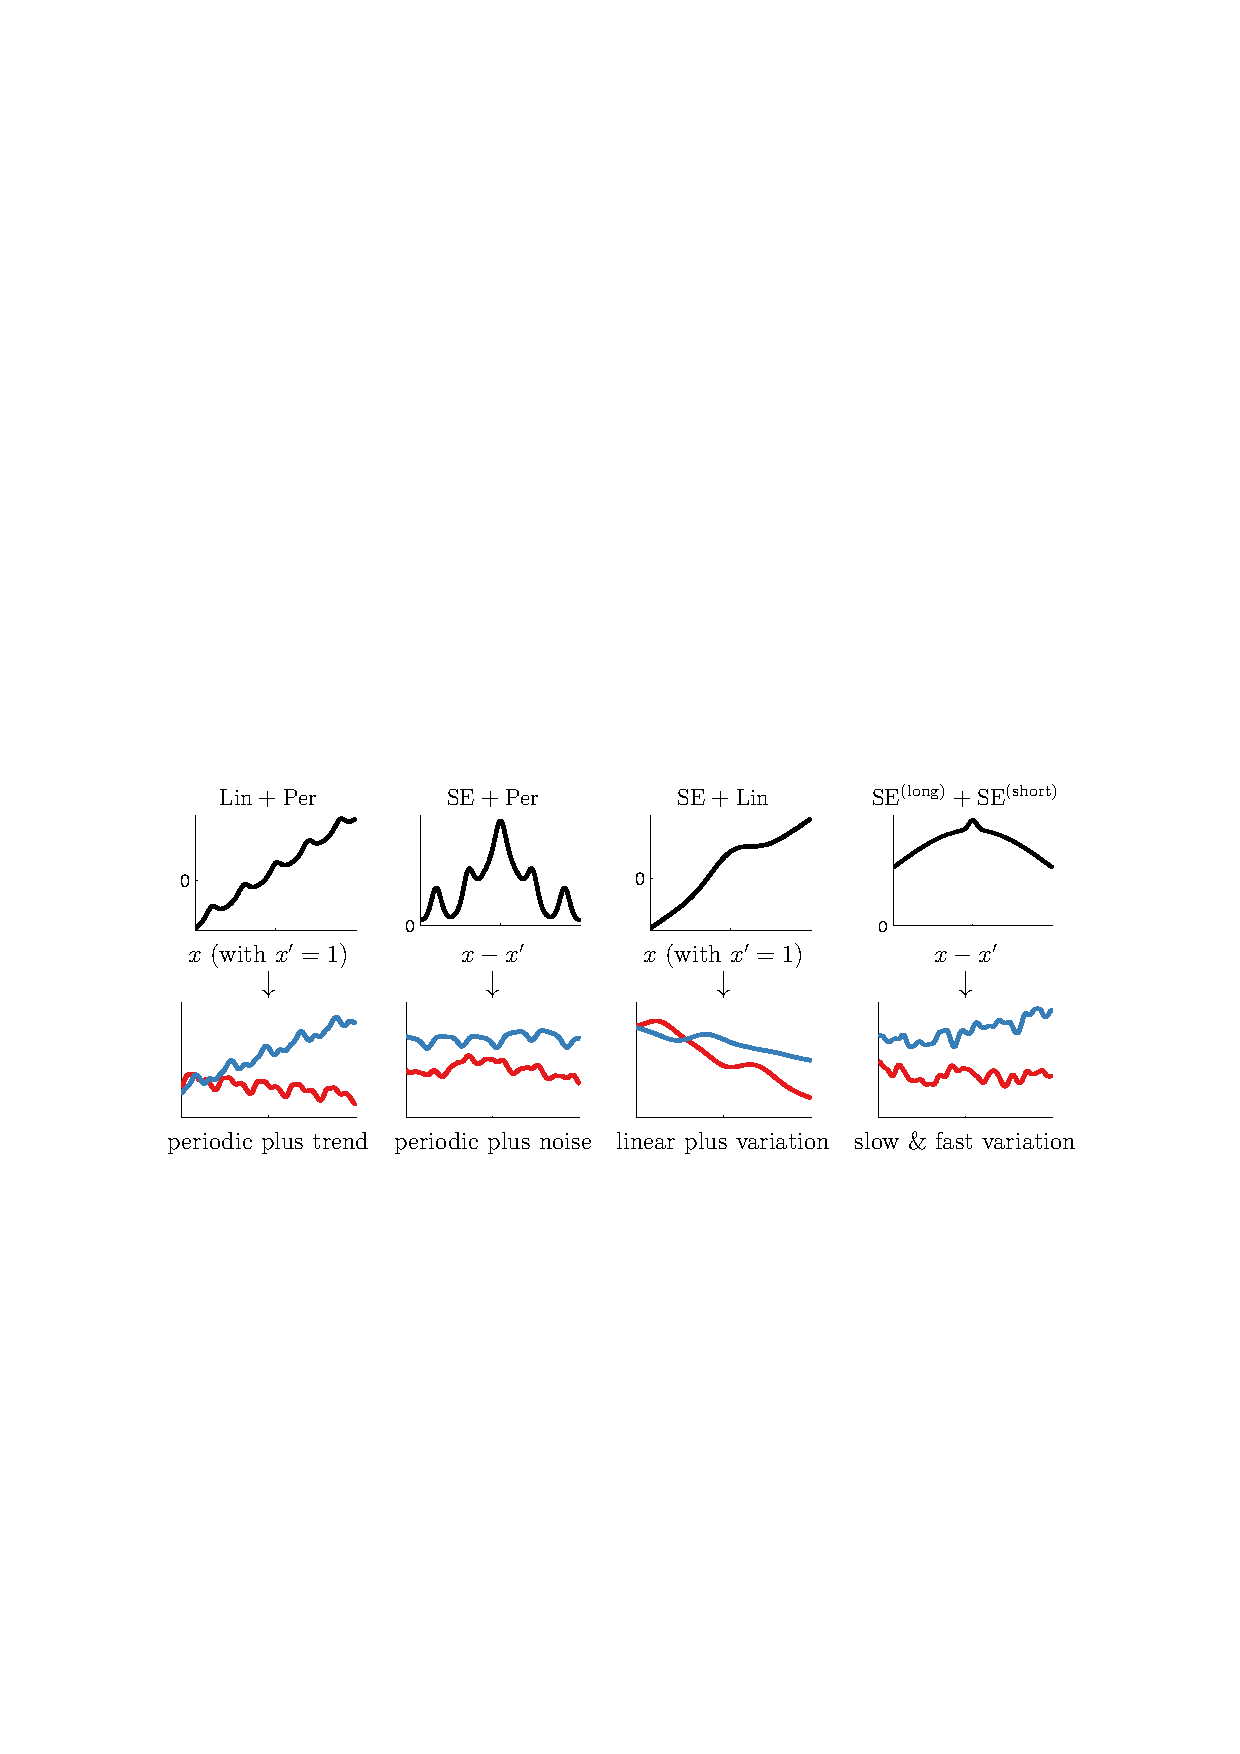
\includegraphics[width=0.95\textwidth]{figures/kernel1}
	\caption{Sum of different kernels \label{fig:ker1}}
\end{figure}
\vspace{0.5cm}
\begin{figure}[h]
\center
	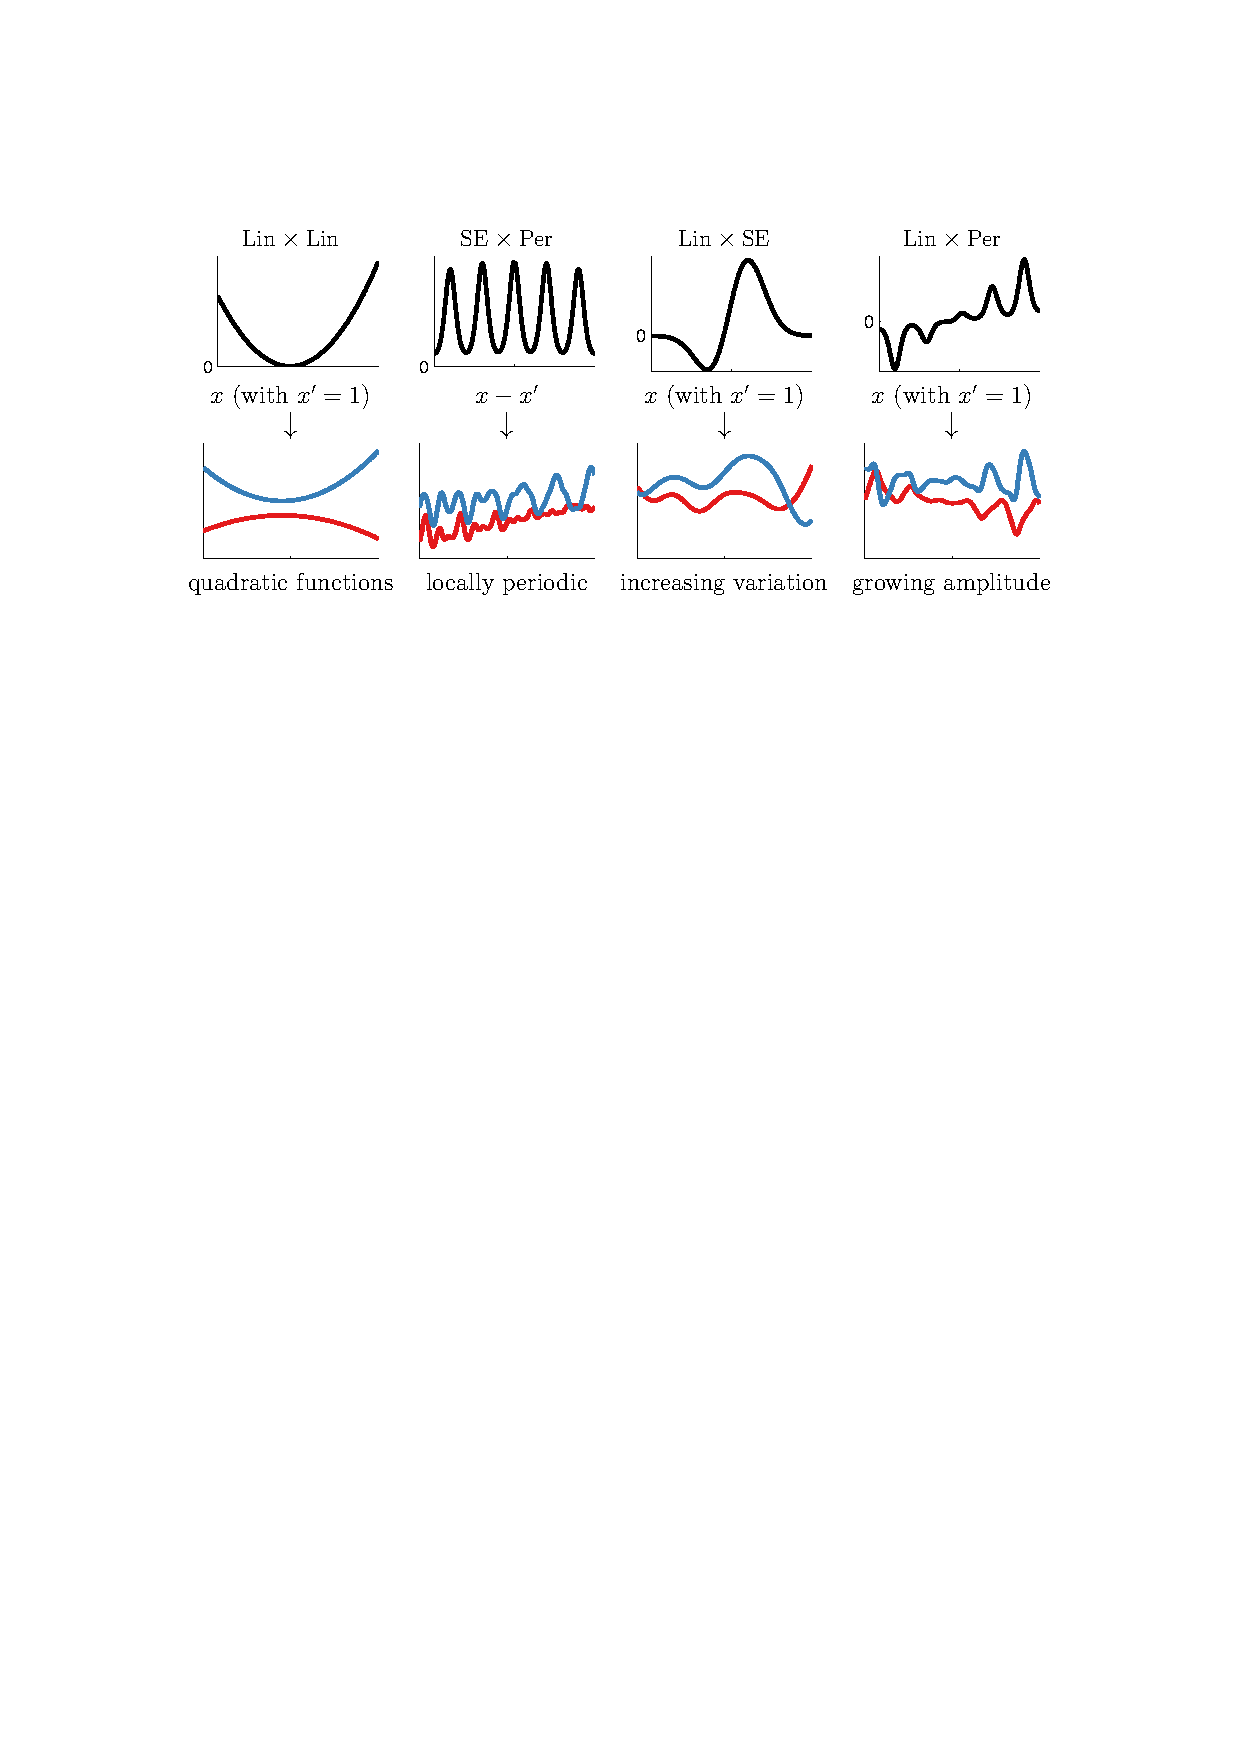
\includegraphics[width=0.95\textwidth]{figures/kernel2}
	\caption{Product of different kernels \label{fig:ker2}}
\end{figure}


	
	\newpage
	\chapter{Ensamble Methods}
	\begin{tcolorbox}
\begin{tabular}{ll}
	$(x, y)$ & a random example \\
	$Z$ & a random training set \\
	$Z_1, \cdots Z_M$ & bootstrap sets from $Z$ \\
	$b$ & a base model trained on a bootstrap set \\
	$b^{(M)}$ & an ensemble model trained via bagging on $M$ bootstrap sets
\end{tabular}
\end{tcolorbox}

\section{Bagging}
In bagging methods, each classifier trained on a different bootstrap sample of the
training data, and the final predictions given by the majority voting.
\begin{definition}[Bagging]
Bagging = Bootstrap + Aggregation. For a training set $Z$,
\begin{enumerate}
	\item Draw $M$ bootstrap datasets, $Z_1, \cdots Z_M$, where $Z_i \subset Z$;
	\item Train $M$ base models, $b^{(1)}, \cdots, b^{(M)}$, independently;
	\item Aggregate base models with
	$$
	\hat{b}(\bfx) = \left\{ \begin{array}{ll} \displaystyle \frac{1}{M}\sum_{t \leq M} b^{(t)}(\bfx) & \mathrm{regression} \\ \displaystyle \mathrm{vote}\left\{ b^{(1)}, \cdots, b^{(M)} \right\} & \mathrm{classification}   \end{array} \right.
	$$
\end{enumerate}
\end{definition}
\begin{theorem}[Variance Reducing]
	For $\bfx \in X$, if $range(y) := \max y - \min y < \infty$, then there is a sufficiently large $M$ s.t.
	\begin{align}
		\E{Z, Z'_1,\cdots ,Z'_M, y \mid \bfx}{(y - b^{(M)}(\bfx))^2} \leq \E{Z, Z', y \mid \bfx}{(y - b(\bfx))^2}
	\end{align}
\end{theorem}
\textit{Proof Sketch.} \marginpar{\footnotesize See lecture slide 9.}
\begin{align}
	\E{Z, Z', y \mid \bfx}{(y - {b}(\bfx))^2} & = \E{Z, Z', y \mid \bfx}{(y - \E{Z,Z'}{b(\bfx)} + \E{Z,Z'}{b(\bfx)} - b(\bfx))^2} \\
	& = \E{Z, Z', y\mid \bfx}{(y - \E{Z, Z'}{b(\bfx)})^2} + \underbrace{\E{Z, Z'}{(\E{Z, Z'}{b(\bfx)} - b(\bfx)^2}}_{Var[b(\bfx)] \geq 0} \\
	& \geq \E{Z, Z'_1,\cdots ,Z'_M, y\mid \bfx}{(y - \E{Z, Z'}{\hat{b}(\bfx)})^2}
\end{align} \myqed

\remark The main differences between bagging and boosting:
\begin{itemize}
	\item Bagging builds learners independently, while boosting tries to add new models that do well where previous models fail.
	\item Bagging uniformly samples data, while boosting samples data based on weights.
	\item Bagging uses majority voting, while boosting uses weighted voting (more weight to those with better performance on training data).
	\item Boosting tries to reduce both bias and variance; while bagging only solve the over-fitting problem (high variance).
\end{itemize}

\section{Boosting}
\subsection{AdaBoost}
\begin{itemize}
	\item AdaBoost = Adaptive Boosting
	\item Sequentially add \textit{week} predictors to the ensemble, where each new predictor \textbf{improves} its predecessor by paying more attention to the hard cases.
	\item Final prediction is made via a weighted majority voting scheme.
\end{itemize}

Given the training samples $\{(\bfx_1, y_1), \cdots , (\bfx_n, y_n)\} \in \cX \times \{-1, +1 \} $, and the base model $b(\bfx): \cX \rightarrow \{-1, +1 \}$, the AdaBoost algorithm is shown in Alg.~\ref{alg:adaboost}.

\begin{algorithm}[H]
\setstretch{1.35}
\caption{AdaBoost method (from Slides 6 \& Toturial 8) \label{alg:adaboost}}
\SetAlgoLined
 $w_i^{(t)} = 1/n$ \textbf{for} $i=1,\cdots,n$\;
 \For{$t = 1, \cdots, M$}{
  $b_t(\bfx) = \displaystyle \argmin_{b} \sum_{i\leq n} w_i^{(t)} \Ind{y_i \neq b(\bfx_i)} $\;
  $\epsilon_t = \displaystyle \left(\sum_{i \leq n} w_i^{(t)} \Ind{y_i \neq b_t(x_i)}\right) \bigg/ \left(\sum_{i \leq n} w_i^{(t)}\right) $\Comment*[r]{weighted error rate}
  $\alpha_t = \displaystyle  \log{\frac{\textstyle 1-\epsilon_t}{\textstyle \epsilon_t}}$\Comment*[r]{correct and wrong samples both get half of the weights}
  $w_i^{(t+1)} = w_i^{(t)} \exp\left( \alpha_t \Ind{y_i \neq b_t(\bfx_i)} \right) $\;
 }
\KwOut{ $\widehat{b}(x) = \displaystyle \sign\left(\sum_{t \leq M} \alpha_t b_t(\bfx) \right)$, $\forall \bfx \in \cX$
}
\end{algorithm}
Note that there is another version of AdaBoost typically found in literatures. The difference lies in how to handle correct samples. In the previous version, correct samples will have unchanged weights; whereas in the second version, they will have weights of $\exp(-\alpha_t)$.

\begin{algorithm}[H]
\setstretch{1.35}
\caption{AdaBoost method (another version) \label{alg:adaboost2}}
\SetAlgoLined
 $w_i^{(t)} = 1/n$ \textbf{for} $i=1,\cdots,n$\;
 \For{$t = 1, \cdots, M$}{
  $b_t(\bfx) = \displaystyle \argmin_{b} \sum_{i\leq n} w_i^{(t)} \Ind{y_i \neq b(\bfx_i)} $\;
  $\epsilon_t = \displaystyle \sum_{i \leq n} w_i^{(t)} \Ind{y_i \neq b_t(x_i)} $\Comment*[r]{weighted error rate}
  $\alpha_t = \displaystyle  \onehalf \log{\frac{\textstyle 1-\epsilon_t}{\textstyle \epsilon_t}}$\Comment*[r]{note the additional $1/2$}
  $Z_t = 2 \sqrt{\epsilon_t (1 - \epsilon_t)}$\Comment*[r]{normalizer}
  $w_i^{(t+1)} = w_i^{(t)} \exp\left( -\alpha_t y_i b_t(\bfx_i) \right) /\, Z_t$\;
 }
\KwOut{ $\widehat{b}(x) = \displaystyle \sign\left(\sum_{t \leq M} \alpha_t b_t(\bfx) \right)$, $\forall \bfx \in \cX$
}
\end{algorithm}
\remark Here we only consider binary classification problem, where the base models are assumed to have accuracy higher than 50\%. Thus, Line 5 will not decrease the weight of mis-classified samples.

\begin{theorem}[Empirical Error of AdaBoost]The empirical error of the classifier returned by AdaBoost verifies
$$
\widehat{\mathrm{Err}}(b) \leq \exp\left[ -2 \sum_{t \leq M}(\onehalf - \epsilon_t)^2 \right].
$$
\end{theorem}
\begin{proof}
\begin{equation}
		\widehat{\mathrm{Err}}(b)=\frac{1}{n} \sum_{i=1}^{n} \Ind{y_{i} \neq b(\bfx_{i})} \leq \frac{1}{n} \sum_{i=1}^{n} e^{-y_{i} b(\bfx_{i})}=\frac{1}{n} \sum_{i=1}^{n}\left[n \prod_{t=1}^{M} Z_{t}\right] w^{(M+1)}_{i}=\prod_{t=1}^{M} Z_{t}.
\end{equation}

\end{proof}

\subsection{Gradient Boosting}
Gradient Boosting is yet another popular and efficient approach. It uses gradients (or residuals) instead of sample weights. The final predictions are made from weighted sum of weak models. It works for arbitrary differentiable loss functions $L(y, f(\bfx))$.

\begin{algorithm}[H]
\setstretch{1.35}
\caption{Gradient Boosting \label{alg:gb}}
\SetAlgoLined
 \For{$t = 1, \cdots, M$}{
  Compute gradient: $g_t(\bfx_i) = \displaystyle - \left[ \frac{\partial L(y_i; f(\bfx_i))}{\partial f(\bfx_i)} \right]_{f = \widehat{f}_{t - 1}} \;
  \forall i \leq n $\;
  Fit weak learner to the gradients: $\displaystyle h_t = \argmin_h \sum_{i\leq n}(-g_t(\bfx_i) - h(\bfx_i))^2$\;
  Fit the step length via line search: $\displaystyle \beta_t = \argmin_\beta \sum_{i \leq n} L(y_i,  \widehat{f}_{t - 1}(\bfx_i) + \beta h_t(\bfx_i)) $\;
  Update $ \widehat{f}_{t}(\bfx) =  \widehat{f}_{t - 1}(\bfx) + \beta_t h_t(\bfx)$\;
 }
\KwOut{ $\widehat{f}_{M}(\bfx)$
}
\end{algorithm}

%\subsection{From the stage-wise perspective (Exercise 6)}
%\begin{algorithm}[H]
%\setstretch{1.3}
% \caption{Stage-wise AdaBoost}
%\SetAlgoLined
% $w_i^{(t)} = 1/n$ \textbf{for} $i=1,\cdots,n$\;
% \For{$t = 1, \cdots, M$}{
%  $f_t(x) = \argmin_{b} \sum_{i\leq n} w_i^{(t)} \Ind{y_i \neq b(x_i)} $\;
%  $\epsilon_t = \sum_{i \leq n} w_i^{(t)} \Ind{y_i \neq f_t(x_i)} \ \slash \sum_{i \leq n} w_i^{(t)} $\;
%  $\alpha_t = \log{\frac{\textstyle 1-\epsilon_t}{\textstyle \epsilon_t}}$\;
%  $w_i^{(t+1)} = w_i^{(t)} \exp\left( \alpha_t \Ind{y_i \neq f_t(x_i)} \right) $\;
% }
%\KwOut{ $\hat{c}(x) = \sign\left(\sum_{t \leq M} \alpha_t f_t(x) \right)$, $\forall x \in \R^D$
%}
%\end{algorithm}

\subsection{Theoretical Insights}
\subsubsection{Forward Stage-wise Additive Estimator with the Exponential Loss}
Let $L(y, y') = \exp(-y y')$ be an exponential loss, then AdaBoost can be translated into the following form.

\begin{algorithm}[h]
\setstretch{1.35}
\caption{AdaBoost (FSAE explanation) \label{alg:fsae}}
\SetAlgoLined
$f_0(\bfx) = 0$, for all $\bfx \in \R^D$\;
 \For{$t = 1, \cdots, M$}{
 	$\displaystyle (\alpha_t, b^{(t)}) = \argmin_{\alpha, b} \sum_{i = 1}^n L(y_i, \alpha b(\bfx_i), + f_{t-1}(\bfx_i))$\;
 	$f_t(\bfx) = \alpha_t  b^{(t)}(\bfx_i) + f_{t-1}(\bfx_i)) $for all $\bfx \in \R^D$\;
 }
\KwOut{ $\widehat{f}_{M}(\bfx)$
}
\end{algorithm}

The proof of the equivalence can be found in Ex.6 - 1.


\subsubsection{AdaBoost trains max-margin classifiers}

	\begin{align}
	b^{(M)}(\bfx) = \sign\left(\sum_{t \leq M} \alpha_t b^{(t)}(\bfx) \right) \qquad w.l.o.g.\ \sum_{t \leq M} \alpha_t = 1
\end{align}

\begin{align}
	margin(\bfx_i) := y_i \sum_{t \leq M}  \alpha_t b^{(t)}(\bfx_i) \longrightarrow 0 \quad ({M \rightarrow \infty})
\end{align}



	
	\newpage
	\chapter{Non-parametric Methods}
	\section{Expectation Maximization (EM)}
The Expectation Maximization (EM) algorithm is one approach to unsupervised, semi-supervised, or lightly supervised learning. Given a model $p$ (parameterized by $\theta$) of observable variables $\bfx_1, \cdots, \bfx_n$ and latent variables $\bfz_1, \cdots, \bfz_m$, EM is an efficient method that \textbf{approximately} solves the following optimization problem,
\begin{equation}
	\theta^* = \argmax_{\theta} \max_{\bfz_1, \cdots, \bfz_n} p(\bfx_1, \cdots, \bfx_n, \bfz_1, \cdots, \bfz_m \mid \theta)
\end{equation}

\begin{definition}[EM Principle]
	Let $\cX = \{\bfx_1, \cdots, \bfx_n\}$ be the observable variables, $\cX_L = \{\bfz_1, \cdots, \bfz_m\}$ be the latent variables. The EM method is to repeat the following procedure until the convergence of $\theta$. \marginpar{\footnotesize Intuitively, EM is to optimize two group of coordinates alternatively. When optimizing one group, the other group is fixed.
	
	This is called ``coordinates descent''.}
	\begin{enumerate}
		\item \textbf{Expectation step}: Calculate a function $Q$ of $\theta$, given  previous-estimated $\theta^{(j)}$,
		$$
Q\left({\theta}; {\theta}^{(j)}\right) := \mathbb{E}_{\mathcal{X}_{L}}\left[L\left(\mathcal{X}, \mathcal{X}_{L} \mid {\theta}\right) \lvert\  \mathcal{X}, {\theta}^{(j)}\right]
$$
Here, $L(\mathcal{X}, \mathcal{X}_{L} \mid {\theta}) = \log p(\mathcal{X}, \mathcal{X}_{L} \mid {\theta})$ is the log-likelihood function.
	\item \textbf{Maximization step}: Estimate new parameter ${\theta}^{(j + 1)}$ by maximizing the function $Q$,
	$$
	\theta^{(j + 1)} = \argmax_\theta Q\left({\theta}; {\theta}^{(j)}\right).
	$$
	\end{enumerate}
\end{definition}
\begin{theorem}[EM's Correctness]
	 EM method is guaranteed to converge to a point with gradient of $0$.	
\end{theorem}
\textit{Proof Sketch.}

\subsection{K-Means Clustering}
\begin{definition}[K-Means Problem]
	Given $d$-dimensional sample vectors $\cX = \{ \bfx_1, \cdots, \bfx_n\}$ and an assignment function $c(\bfx): \R^d \rightarrow \{1, \cdots, k\}$ with prototypes $\bfmu_{c(\cdot)} \in \cY \subset \R^d$. The k-means finds the $c(\cdot)$ and $\cY$ that minimize 
	$$
	R(c, \cY) = \sum_{\bfx \in \cC} \norm{\bfx - \bfmu_{c(\bfx)}}^2_2.
	$$
\end{definition}
The k-means problem is a mixture problem of combinatorial and continuous optimization, which is hard to optimize directly. Practically, K-Means relies on the \textbf{Hard-EM} technique, as shown in Alg.~\ref{alg:kmeans}.

\begin{algorithm}[H]
\setstretch{1.3}
 \caption{K-Means, an example of Hard-EM \label{alg:kmeans}}
\SetAlgoLined
 
 \While{$c(\bfx)$ and $\bfmu_{c}$ keep changing}{
  $c(\bfx) = \argmin_{c \in \{1, \cdots, k\}} \norm{\bfx - \bfmu_c}^2_2$\Comment*[r]{E-step: assign $\bfx$ to the nearest prototypes}
  $\displaystyle \bfmu_\alpha = \frac{1}{|N_\alpha|} \sum_{\bfx \in N_\alpha} \bfx$, where $N_\alpha = \{\bfx\mid c(\bfx) = \alpha\}$
  \Comment*[r]{M-step: update prototypes}
 }
\KwOut{ $c(\bfx), \forall \bfx \in \cX$}
\end{algorithm}

\subsection{Gaussian Mixture Models (GMM)}
In mixture models, data are assumed to be generated by a mixture of distribution $p(\bfx \mid \theta)$. Mixture models are generative, which tries to describe all the data. 
\begin{definition}[GMM]
	A Gaussian mixture is a convex combination of $k$ Gaussian distributions,
	$$
p\left(\mathbf{x} \mid \pi_{1}, \ldots, \pi_{k}, {\theta}_{1}, \ldots, {\theta}_{k}\right)=\sum_{c \leq k} \pi_{c} p\left(\mathbf{x} \mid {\theta}_{c}\right), \where p(\bfx \mid \theta_c) = \cN(\bfx; \mu_c, \Sigma_c).
$$
Here, $\pi_c > 0$ is the mixture weight, denoting the prior probability that a sample is generated by the mixture Gaussian component $c$ with parameters $\theta_c = \{\mu_c, \Sigma_c \}$.
\end{definition}

To estimate parameters $\theta_c$, we can maximize its likelihood of sample feature vectors $\cX = \{ \bfx_1, \cdots, \bfx_n\}$. The log-likelihood is often computationally preferable, as
\begin{equation}
	L(\cX; \pi_{1}, \ldots, \pi_{k}, {\theta}_{1}, \ldots, {\theta}_{k}) = \sum_{\bfx \in \cX} \log \sum_{c\leq k}{\pi_c p(\bfx \mid \theta_c)}.
\end{equation}
However, to directly maximize it is still intractable, because the logarithm within the sum makes it a non-convex problem. Alg.~\ref{alg:gmm} shows the Soft-EM method that solves the GMM problem.

\begin{algorithm}[H]
\setstretch{1.4}
 \caption{GMM, an example of Soft-EM \label{alg:gmm}}
\SetAlgoLined
 
 \While{$c(\bfx)$ and $\bfmu_{c}$ keep changing}{
  $\gamma_{\bfx, c} = \displaystyle \frac{p(\bfx \mid c, \theta^{(j)}\ p(c \mid \theta^{(j)})}{p(\bfx \mid \theta^{(j)})}$\Comment*[r]{E-step: soft-assign sample $\bfx$ to clusters}
  \vspace{1mm}
  $\displaystyle \bfmu_c^{(j + 1)} = \frac{\sum_{\bfx} \gamma_{\bfx, c}\, \bfx}{\sum_\bfx \gamma_{\bfx, c}}$,\ \ $\displaystyle \Sigma_c^{(j + 1)} = \frac{\sum_{\bfx} \gamma_{\bfx, c} (\bfx - \bfmu_c)^2}{\sum_\bfx \gamma_{\bfx, c}}$\Comment*[r]{M-step: update parameters}
  \vspace{2mm}
  $\displaystyle \pi_c^{(j + 1)} = \frac{1}{|\cX|}\sum_{\bfx} \gamma_{\bfx, c}$\;
 }
\KwOut{ $c(\bfx), \forall \bfx \in \cX$}
\end{algorithm}
Here, $\gamma_{\bfx, c}$ is the ``responsible probability'', denoting the probability that $\bfx$ belongs to component $c$, i.e. $\gamma_{\bfx, c} = p(y = c | \bfx, \theta)$. 

Next, we will proof the correctness of 
\begin{proof}
	
\end{proof}
\section{Dirichlet Process}

\begin{definition}[Beta Distribution]
	$$
	\mathrm{Beta}(\theta; a, b) = \frac{1}{\beta(a, b)} \theta^{a-1} (1-\theta)^{b - 1}, \where \beta(a, b) = \frac{\Gamma(a)\Gamma(b)}{\Gamma(a + b)}
	$$
	Here, $\Gamma(z)$ is the Gamma function, $\Gamma(z) = \int_0^\infty x^{z-1} e^{-x} \dx$.
\end{definition}
\remark Beta distribution is the probability $\theta$ of a Bernoulli process after observing $a - 1$ successes and $b - 1$ failures. 

Please note that the Binomial distribution $\mathrm{Bin}(k; n, p) = C(n, k) p^k (1-p)^{n-k}$ is a function of number of success trials $k \in \mathbb{N}$, while the Beta distribution $\mathrm{Beta}(\theta; a, b)$ is a function of the success probability $\theta \in [0, 1]$.

\begin{definition}[Dirichlet Distribution]
	Dirichlet distribution is the multivariate generalization of the beta distribution. Given $\bfx = \{ x_1, \cdots, x_n \}\ (x_i \in [0, 1])$ and $\boldsymbol{\alpha} = \{ \alpha_1, \cdots, \alpha_n \}\ (\alpha_i > 0)$,
	$$
	\mathrm{Dir}(\bfx; \boldsymbol{\alpha}) = \frac{1}{\beta(\boldsymbol{\alpha})} \prod_{k \leq n} x_k^{\alpha_k - 1}, \where \beta(\boldsymbol{\alpha}) = \frac{\prod_{k\leq n} \Gamma(\alpha_k)}{\Gamma(\sum_{k\leq n} \alpha_k)}
	$$
\end{definition}

\begin{definition}[Dirichlet Process]
	A Dirichlet Process $DP(\alpha, H)$ is a stochastic process whose sample paths are probability distributions on a space $\Theta$. Here, $\alpha > 0$ is the ``concentration parameter'', and $H$ is the base measure on $\Theta$. For any measurable finite partition of $\Theta$, denoted by $\{B_1, \cdots, B_n\}$, if $G\sim DP(\alpha, H)$, then 
	$$
	(G(B_1), \cdots, G(B_n)) \sim \mathrm{Dir}(\alpha H(B_1), \cdots, \alpha H(B_n))
	$$
\end{definition}
\remark Note that $H$ is continuous, so the probability that any two samples are equal is precisely zero. However, $G$ is a discrete distribution, made up of a countably infinite number of point masses, and thus there is a non-zero probability of two samples colliding.

\begin{theorem}[De Finetti's Theorem]
Let $(X_1, X_2, \cdots)$ be an infinitely exchangeable sequence of random variables. Then, $\forall n$:
$$
p(X_1, \cdots, X_n) = \int (\prod_i p(x_i \mid G))\ \mathrm{d} P(G),
$$
for some random variable $G$.	
\end{theorem}
\remark An infinitely exchangeable sequence can be represented by a product of conditionally independent random variables.

\subsection{Stick-Breaking Process}
Stick-breaking process provides a constructive way to draw samples from $DP(\alpha, H)$.

\begin{algorithm}[H]
\setstretch{1.3}
 \caption{Stick-Breaking Process}
\SetAlgoLined
 
 \For{$k = 1, 2 \cdots$}{
  $\beta_k \sim \mathrm{Beta}(1, \alpha)$\;
  $\rho_k = \beta_k \prod_{i=1}^{k - 1} (1 - \beta_i) $
  \Comment*[r]{alternatively, $\rho_k = \beta_k (1 - \sum_{i=1}^{k-1}\rho_i) $}
  $\theta_k \sim H$\;
 }
\KwOut{ $G(\theta) = \sum_{k=1}^\infty \rho_k \delta_{\theta_k}(\theta) $
}
\end{algorithm}

Here, $\delta_t(\theta)$ is the Dirac function.

\begin{definition}[GEM Distribution]
	The $\{\rho_1, \rho_2, \cdots\}$'s distribution in the Stick-breaking process is called GEM distribution, named after Griffiths-Engen-McCloskey.
	$$
	\{\rho_1, \rho_2, \cdots\} \sim \mathrm{GEM}(\alpha)\quad \Longrightarrow \quad \forall k, \rho_k = \beta_k (1 - \sum_{i=1}^{k-1}\rho_i), \where \beta_k \sim \mathrm{Beta}(1, \alpha).
	$$
\end{definition}

\subsection{Chinese Restaurant Process (CRP)}
The Chinese restaurant process (CRP) is a metaphor of Dirichlet process.
\begin{definition}[CRP]
Let $\cP = \{\tau_1, \cdots, \tau_k \}$ denote a $k$-partition over the integers $\{1, \cdots, n\} $. The partition $\cP$ represents the table assignment, i.e., $|\tau_i|$ is the number of people sitting at table $i$.

	When a new person arrives, he can either join an existing table $i$ $(1 \leq i \leq k)$ with probability proportional to $|\tau_i|$, or start a new table with probability proportional to $\alpha$.
	More formally,
$$
p(n + 1 \text{ joins table } \tau \mid \cP) = \left\{ \begin{aligned}
	\frac{|\tau|}{\alpha + n} & \quad \tau \in \cP, &\quad (\text{to join table } i )\\
	\frac{\alpha}{\alpha + n} & \quad \tau \notin P. &\quad (\text{to start a new table})
\end{aligned}\right.
$$
\end{definition}
\textbf{Remark} The larger the $\alpha$ is, the greater the number of clusters (tables) is.

\begin{property}[CRP is Exchangeable]
	No matter in which order people come, the probability of a given partition $\cP$ is the same, i.e.,  
	\begin{equation}
		p(\cP) = \frac{\alpha^k}{\alpha (\alpha+1)\cdots (\alpha + n - 1)} \prod_{1 \leq i \leq k} (|\tau_i| - 1)!
	\end{equation}
\end{property}

\begin{property}[Number of Occupied Tables in CRP]
	The number of occupied tables in CRP after $N$ customers is
	\begin{equation}
		S(N) = \sum_{1 \leq i \leq N} \frac{\alpha}{\alpha + i - 1} \sim \mathcal{O}(\alpha\log N).
	\end{equation}
\end{property}
\begin{proof}
Let $\cP_i$ be the partition after $i$ customers.
The The number of occupied tables after $N$ customers can be written as, 
\begin{align}
	S(N) & = \E{}{\sum_{1 \leq i \leq N} \Ind{\tau_i \notin \cP_i} } \\
	& = \sum_{1 \leq i \leq N} \E{}{\Ind{\tau_i \notin \cP_i}} \\
	& = \sum_{1 \leq i \leq N} p(\mathrm{start\ a\ new\ table} \mid n = i) \\
	& = \sum_{1 \leq i \leq N} \frac{\alpha}{\alpha + i - 1}
\end{align}
\end{proof}

\begin{exercise}[Ex.8-2: Dirichlet Process]
	Consider the following algorithm for sampling from the Dirichlet process with base distribution $F_0$ and concentration parameter $\alpha$. 
	\begin{enumerate}
		\item Draw the first sample $X_1 \sim F_0$.
		\item For $i = 2, 3, \cdots $, draw
\begin{equation}
X_{i} \mid Z_{1}, \ldots, X_{i-1}=\left\{\begin{array}{ll}
X \sim \hat{F}_{i-1}, & \text { with probability } p=\frac{i-1}{\alpha+i-1} \\
X \sim F_{0}, & \text { with probability } p=\frac{\alpha}{\alpha+i-1}
\end{array}\right.
\end{equation}
where $\widehat{F}_{i - 1}$ is the empirical distribution of $X_1, \cdots , X_{i - 1}$.
	\end{enumerate}
Find the asymptotics of the expected number of distinct samples drawn, as a function of the total number of
samples drawn: $X_1, \cdots , X_n$. Or equivalently, the number of occupied tables in the Chinese restaurant process
metaphor.
\end{exercise}
\begin{sol}
Note that the base distribution $F_0$ is a continuous, so the probability of sampling a sample $X'$ that equal to any number of finite sample $X_1, \cdots X_i$ is $0$. The distinct sample after $n$ samples drawn, 
\begin{align}
	S(n) & = \E{}{\sum_{i \leq n} \Ind{x_i\cup \{X_1, \cdots, X_{i-1} \} = \phi} } \\
	& = \sum_{i \leq n} p(X_i \sim F_0)\ p(x_i\cup \{X_1, \cdots, X_{i-1} \} = \phi  \mid X_k \sim F_0) \\
	& = \sum_{i \leq n} \frac{\alpha}{\alpha + i - 1}
\end{align}

Then, it is easy to prove that $S(n) \sim O(\alpha \log n)$.

%\begin{align}
%\lim_{n \rightarrow +\infty} \frac{S(n)}{\alpha \log n} = 
%\end{align}
\end{sol}

\subsection{DP Mixture Model}
\begin{definition}
Let $\Theta$ be a set that parameterizes a set of probability distributions, and fix a base measure $H$ on $\Theta$. Here, we assume that $\Theta = \R $ and $H = \cN(\mu_0, \sigma_0)$ for some fixed $\mu_0 \in \R, \sigma_0 \in \R_+$. The DP Mixture model is defined as
	\begin{itemize}
		\item Probabilities of clusters (``mixture weights''): $\boldsymbol{\rho} = (\rho_1, \rho_2, \cdots) \sim GEM(\alpha)$,
		\item Centers of the clusters: $\mu_k \sim \cN(\mu_0, \sigma_0), \ k = 1,2,\cdots $,
		\item Assignments of data points to clusters: $z_i \sim \mathrm{Categorical}(\rho), \ i = 1,2,\cdots $
	\end{itemize}
\end{definition}

\subsection{Latent Dirichlet Allocation (LDA)}
Latent Dirichlet Allocation (LDA) is one of the most popular non-parametric model.
\begin{definition}
	Given $K$ topics and $V$ words in the vocabulary, for $M$ documents with $N$ words each.
	\begin{itemize}
		\item Distribution of topics in document $d$: $ \boldsymbol{\theta}_d \sim \mathrm{Dir}(\boldsymbol{\alpha});$
		\item What topic the word $w$ belongs to in document $d$: $z_{d, w} \sim \mathrm{Categorical}(\boldsymbol{\theta}_d); $
		\item Distribution of words in topic $k$: $ \boldsymbol{\psi}_k \sim \mathrm{Dir}(\boldsymbol{\beta}); $
		\item What word $w$ in document $d$: $w_{d} \sim \mathrm{Categorical}(\boldsymbol{\psi}_{z_{d, w}}) $
	\end{itemize} 
\end{definition}

\section{Sampling Methods}
\subsection{Markov-chain Monte Carlo (MCMC)}
Markov-chain Monte Carlo (MCMC) is a powerful framework, allowing sampling from a large class of distributions.

\begin{algorithm}[h]
\setstretch{1.25}
 \caption{MCMC Sampling}
\SetAlgoLined
 
 \For{$\tau = 1, 2 \cdots$}{
  $\bfz^* \sim p(\bfz \mid \bfz^{(\tau)})$\Comment*[r]{proposal distribution}
  $\alpha \sim \mathrm{Uniform}(0,1) $\Comment*[r]{acceptance threshold}
  \eIf{$A(\bfz^*, \bfz^{(\tau)}) = p(\bfz^*)\ p(\bfz^{(\tau)} \mid \bfz^*) > \alpha$}{$\bfz^{(\tau + 1)} = \bfz^*$}{$\bfz^{(\tau + 1)} = \bfz^{(\tau)}$}
 }
\KwOut{ $ \{\bfz^{(1)}, \bfz^{(2)}, \cdots \} $
}
\end{algorithm}

\subsection{Gibbs Sampling}
However, the converge of MCMC is typically slow. Gibbs sampling is a simple and faster method that samples one random variable from conditional distribution at a time, while the remaining variables fixed to their current values.
The theory of MCMC guarantees that the stationary distribution of the samples generated is the target joint posterior. 

\begin{algorithm}[H]
\setstretch{1.25}
 \caption{Gibbs Sampling}
\SetAlgoLined
 Initialize: $ \bfz^{(0)} \sim q(\bfz)$\;
 \For{$\tau = 1, 2 \cdots$}{
	$\bfz_{1}^{(\tau)} \sim p\left(Z_{1}=\bfz_{1} \mid Z_{2}=\bfz_{2}^{(\tau-1)}, Z_{3}=\bfz_{3}^{(\tau-1)}, \cdots, Z_{D}=\bfz_{D}^{(\tau-1)}\right)$\;
	$\bfz_{2}^{(\tau)} \sim p\left(Z_{2}=\bfz_{2} \mid Z_{1}=\bfz_{1}^{(\tau)}, Z_{3}=\bfz_{3}^{(\tau-1)}, \cdots, Z_{D}=\bfz_{D}^{(\tau-1)}\right)$\;
	$\vdots$\\
	$\bfz_{D}^{(\tau)} \sim p\left(Z_{D}=\bfz_{D} \mid Z_{1}=\bfz_{2}^{(\tau)}, Z_{2}=\bfz_{2}^{(\tau)}, \cdots, Z_{D-1}=\bfz_{D-1}^{(\tau)}\right)$\;

 }
\KwOut{ $ \{\bfz^{(1)}, \bfz^{(2)}, \cdots \} $
}
\end{algorithm}

\begin{property}[Gibbs Samples is a Special Case of Metropolis-Hastings]
	We can view the Gibbs sampling as a special case of Metropolis-Hastings, where the acceptance of Gibbs' samples is always $1$.
\end{property}
\begin{proof}
Let $\bfz_{k}$ denotes the the sample's projection at $k$-th dimension and $\bfz_{\backslash k}$ denotes the sample's projection at dimensions other than $k$. In Gibbs sampling, we have $ q_k(\bfz^* \mid \bfz) = p(\bfz_k^* \mid \bfz_{\backslash k})$ (every time we sample one variable, and fix others). Therefore,
	\begin{align}
		A\left(\bfz^{*}, \bfz\right)=\frac{p\left(\bfz^{*}\right) q_{k}\left(\bfz \mid \bfz^{*}\right)}{p(\bfz) q_{k}\left(\bfz^{*} \mid \bfz\right)}=\frac{p\left(z_{k}^{*} \mid \bfz_{\backslash k}^{*}\right) p\left(\bfz_{\backslash k}^{*}\right) p\left(z_{k} \mid \bfz_{\backslash k}^{*}\right)}{p\left(z_{k} \mid \bfz_{\backslash k}\right) p\left(\bfz_{\backslash k}\right) p\left(z_{k}^{*} \mid \bfz_{\backslash k}\right)}=1
	\end{align}
\end{proof}

\newpage

\begin{table}[hbp]
\center
\caption{Summary of some useful sampling methods}
\begin{tabular}{l l l l}
\toprule
\textbf{Method} & \textbf{Metropolis} & \textbf{Metropolis-Hastings} & \textbf{Gibbs} \\
\midrule
Proposal dist. & $q(\bfz \mid \bfz^{(\tau)})$ & $q(\bfz \mid \bfz^{(\tau)})$ & $p(\bfz_k \mid \bfz_{\backslash k})$ \\
Assumption & $q(\bfz_A \mid \bfz_B) = q(\bfz_B \mid \bfz_A)$ & - & -  \\
Accept prob.  & $
\min \left\{1, \frac{\displaystyle \tilde{p}\left(\mathbf{z}^{\star}\right)}{\displaystyle \tilde{p}\left(\mathbf{z}^{(\tau)}\right)}\right\}
$ & $
\min \left\{1, \frac{\displaystyle \tilde{p}\left(\mathbf{z}^{\star}\right) q_{k}\left(\mathbf{z}^{(\tau)} \mid \mathbf{z}^{\star}\right)}{\displaystyle \tilde{p}\left(\mathbf{z}^{(\tau)}\right) q_{k}\left(\mathbf{z}^{\star} \mid \mathbf{z}^{(\tau)}\right)}\right\} \ 
$ & $1$ \\
$A_{k}\left(\mathbf{z}^{\star}, \mathbf{z}^{(\tau)}\right)$ & & & \\
\bottomrule
\end{tabular}
\end{table}
	
	\newpage
	\chapter{Deep Learning}
	\section{Neural Network}
\begin{definition}
A $d$-layer neural network (NN) is defined as the composition of the following components:
	\begin{itemize}
		\item Linear functions $L(\bfx) = \bfW \bfx + b: \R^{n} \rightarrow \R^{m}$, $\bfW \in \R^{n \times m}, b \in \R$;
		\item Activation function $\alpha(\bfx): \R^{m} \rightarrow \R^{m}$.
	\end{itemize}
	alternatively applied to the input data $\bfx \in \cX$, i.e.,
	$$
	NN(\bfx) = \alpha^{(d)} \circ L^{(d)} \circ \cdots \circ \alpha^{(1)} \circ L^{(1)}(\bfx).
	$$
	Here, $\circ$ is the composition operator.
\end{definition}

\begin{figure}[h]
\center
	\tikzset{%
  every neuron/.style={
    circle,
    draw,
    minimum size=0.8cm,
    line width=1pt,
    fill=gray!10
  },
  neuron missing/.style={
    draw=none, 
    scale=1,
    text height=0.333cm,
    fill=white,
    execute at begin node=\color{black}$\vdots$
  },
}

\begin{tikzpicture}[x=1.5cm, y=1cm, >=stealth]

\foreach \m/\l [count=\y] in {1,2,3,missing,4}
  \node [every neuron/.try, neuron \m/.try] (input-\m) at (0,2.5-\y) {};

\foreach \m [count=\y] in {1,missing,2}
  \node [every neuron/.try, neuron \m/.try ] (hidden-\m) at (2,2-\y*1.25) {};

\foreach \m [count=\y] in {1,missing,2}
  \node [every neuron/.try, neuron \m/.try ] (output-\m) at (4,1.5-\y) {};

\foreach \l [count=\i] in {1,2,3,n}
  \draw [<-] (input-\i) -- ++(-1,0)
    node [above, midway] {\small $x_\l$};

\foreach \l [count=\i] in {1,n}
  \node [above] at (hidden-\i.north) {\small $h^{(1)}_\l$};

\foreach \l [count=\i] in {1,n}
  \draw [-{>[scale=2.5,length=2,width=6]}] (output-\i) -- ++(1,0)
    node [above, midway] {\small $h^{(2)}_\l$};

\foreach \i in {1,...,4}
  \foreach \j in {1,...,2}
    \draw [-{>[scale=2.5,length=2,width=6]}] (input-\i) -- (hidden-\j);

\foreach \i in {1,...,2}
  \foreach \j in {1,...,2}
    \draw [-{>[scale=2.5,length=2,width=6]}] (hidden-\i) -- (output-\j);

\foreach \l [count=\x from 0] in {\small ${h}^{(0)} = \bfx$, \small ${h}^{(1)} = \alpha^{(1)} \circ L^{(1)}$, \small ${h}^{(2)} = \alpha^{(2)} \circ L^{(2)}$}
  \node [align=center, above] at (\x*2,2) {\l};
\end{tikzpicture}
\vspace{2mm}
\caption{Illustration of a 2-layer neural network}
\label{fig:MLP}
\end{figure}

\subsection{Gradients in NN}
(Omitted here. Please see the Ex. 6 for details.)

\section{Variational Autoencoder}

\subsection{InfoMax Principle}
Let $X$ and $Z$ be a measurement and a representation space, respectively. Let $F = \{\mathrm{enc}_\theta: \theta \in \Theta\}$ be a parametric family of function with $\mathrm{enc}_\theta: X \rightarrow Z$.

\begin{definition}[Mutual Information]
	The mutual information between $X$ and $Z$ is
	$$
	I(X; Z) = \EE_{X,Z}\left[ \log \frac{p(X, Z)}{p(X)p(Z)} \right]
	$$
\end{definition}

\begin{definition}[InfoMax Principle]
	Given a training set $\{x_1, \cdots, x_n\} \in X$, we can do the following approximation 
	$$
	\begin{aligned}
			\argmax_\theta\ I(X; Z) &= \argmax_\theta\ \EE_{X,Z}\left[ \log \frac{p(X, Z)}{p(X)p(Z)} \right] \\
			&= \argmax_\theta\ \EE_{X, Z}\left[ \log p(X \mid Z) \right] - \EE_{X}\left[ \log p(X) \right] \\
			&= \argmax_\theta\ \EE_X \EE_{Z \mid X} \left[ \log p(X_i \mid Z) \right] \\
			&\approx \argmax_\theta\ \sum_{i \leq n} \EE_{Z \mid X} \left[ \log p(X_i \mid Z) \right] 
	\end{aligned}
	$$
	
\end{definition}

\subsection{Variational Autoencoder}

\begin{align}
	& \argmax_{\theta, \theta', \phi}\  \sum_{i \leq n} \log p_{\theta', \theta}(x_i) \\
	=& \argmax_{\theta, \theta', \phi}\  \EE_{Z \sim q_\phi(\cdot \mid x_i)}[\log p_{\theta', \theta}(x_i)] \\
	=& \argmax_{\theta, \theta', \phi}\ \EE_{Z \sim q_\phi(\cdot \mid x_i)}\left[ \log \left(\frac{p_{\theta', \theta}(x_i, Z)}{p_{\theta', \theta}(x_i \mid Z)} \frac{q_\phi(Z \mid x_i)}{q_\phi (Z \mid x_i)} \right) \right] \\
	=& \argmax_{\theta, \theta', \phi}\ \underbrace{\EE_{Z \sim q_\phi(\cdot \mid x_i)}\left[ \log \left(\frac{p_{\theta', \theta}(x_i, Z)}{q_\phi(Z \mid x_i)} \right) \right]}_{\mathrm{ELBO\ of\ } \theta', \theta, \phi } + \underbrace{\EE_{Z \sim q_\phi(\cdot \mid x_i)}\left[ \log \left(\frac{q_\phi(Z \mid x_i)}{p_{\theta', \theta}(Z \mid x_i)} \right) \right]}_{KL\left[ q_\phi( \cdot \mid x_i) \ ||\   p_{\theta, \theta'}(\cdot \mid x_i)\right] \,\geq\, 0}
\end{align}
Note that $p_{\theta', \theta}(x_i, Z) = p_\theta(x_i \mid Z) \, p_{\theta'}(Z)  $. we have 
\begin{equation}
	\mathrm{ELBO} = \underbrace{\EE_{Z \sim q_\phi(\cdot \mid x_i)} [\log p_\theta(x_i \mid Z)]}_{\mathrm{Mutual\ Information:\ } I(X; Z)} + \underbrace{\EE_{Z \sim q_\phi(\cdot \mid x_i)} \left[ \log\left( \frac{p_{\theta'}(Z)}{q_\phi (Z \mid x_i)} \right) \right]}_{-KL\left[ q_\phi( \cdot \mid x_i) \ ||\  p_{\theta'}\right] }
\end{equation}
\remark The Mutual Information term encourage the representation to be infomrative, and KL divergence term tries to disentangle the encoder and decoder. 
\begin{figure}[htbp]
	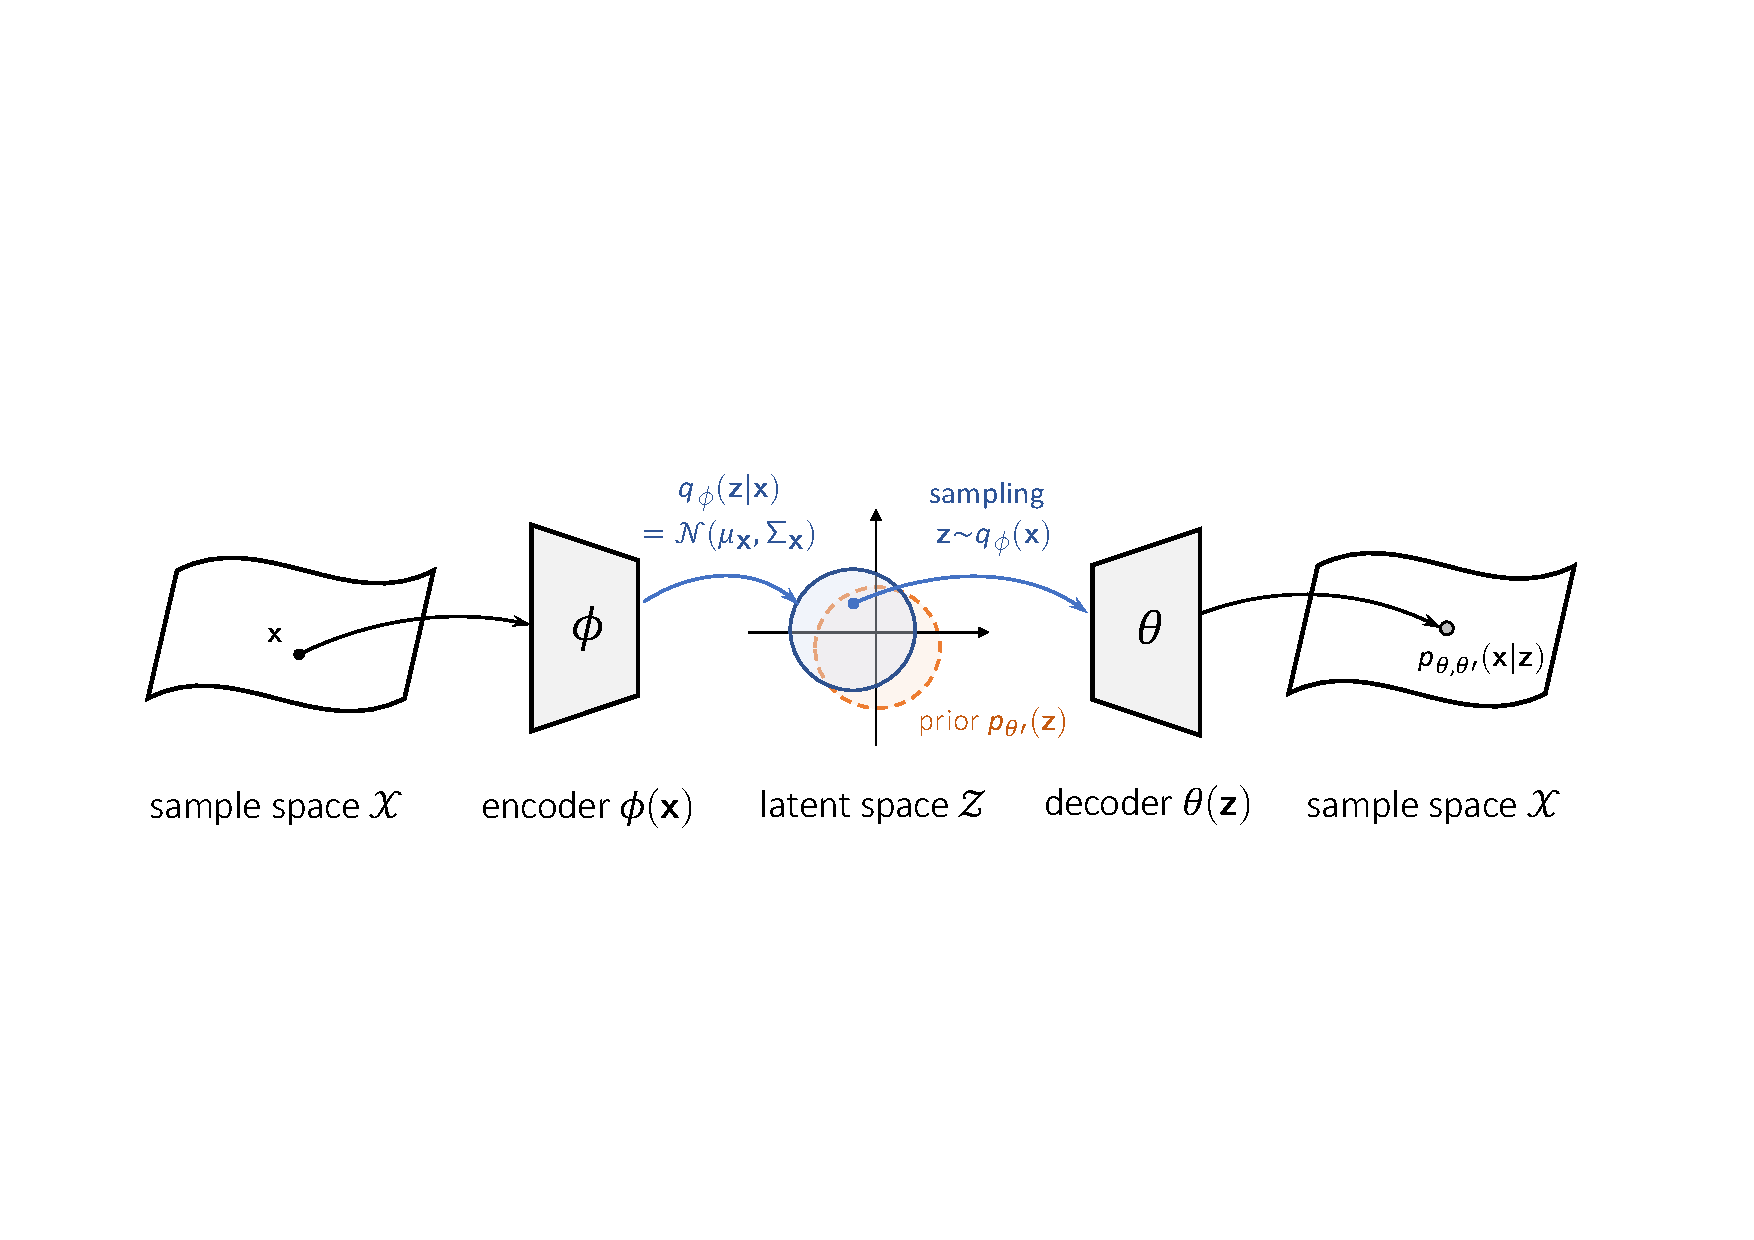
\includegraphics[width=\linewidth]{figures/vae}
	\caption{Illustration for Variational Autoencoder}
\end{figure}

\section{Optimization Methods}
\subsection{Newton's Method}
Newton’s method was originally created to find a root $f(\bfx^*) = 0$ of a given function $f(\bfx)$ via the iteration.
\begin{definition}[Newton's Method] Given a function $f: \cX \rightarrow \R$ and a initial value of $\bfx_0 \in \cX$, Newton’s method finds a root of $f(\bfx^*) = 0$ near $\bfx_0$ by iteration steps as
$$
	\bfx_{n+1} = \bfx_n - \frac{f(\bfx_n)}{f'(\bfx_n)},
$$
where $f'(\bfx)$ denotes the derivative of $f$ with respect to $\bfx$.
\end{definition}
In optimization we are usually interested in finding the minimum of a function. This can be achieved using Newton’s method to find a root of the first derivative $f'(\bfx^*) = 0$, the optimization step then becomes
\begin{equation}
	\bfx_{n+1} = \bfx_n - \frac{f'(\bfx_n)}{f''(\bfx_n)}.
\end{equation}
When applying in the high-dimensions, we have the form as
	\begin{align}
		\bfx_{n + 1} = \bfx_{n} -\mathbf{H}_f^{-1}(\bfx_{n}) \nabla_f(\bfx_{n})
	\end{align}

\begin{property}[Convergence of Newton's Method] \marginpar{\footnotesize A sequence $x_n$ converges with order $m$ towards $x^*$, if there exists a
constant $C$, such that $|x_n-x^*| \leq C |x_n-x^*|^m$} We call a smooth function $f$ with one root $f(x^*) = 0$ has order $k$, if its all derivatives $f^{(i)}(x^*) = 0,$ $\forall i > k$ and $f^{(k)}(x^*) \neq 0$.
	 Newton’s method converges linearly $(m = 1)$ for the function $f$ of order $k > 1$ in a region around the point $x^*$.
\end{property}

\begin{property}[Limits of Newton's Method] Newton's Method does not always work.  For example, it will never converge for $f(x) = \sqrt[3]{x}$ with $x_0 \neq 0$.
\end{property}
\begin{proof}
	Simply, we have
	\begin{equation}
		x_{n+1} = x_n - \frac{f(x_n)}{f'(x_n)} = x_n - \frac{x_n^{1/3}}{x_n^{-2/3} / 3} = -2x_n
	\end{equation}
	It will not converge, since $\lim_{n\rightarrow \infty} |x_n| = \infty, \forall x_0 \neq 0$.
\end{proof}

\subsection{Gradient Descent}
\begin{definition}
In gradient descent (GD), we iteratively estimate $\min_\bfw f(\bfw)$ by computing a sequence of estimates $\bfw^{(0)}, \cdots, \bfw^{(k)}, \cdots$. Each estimate $\bfw^{(k+1)}$ is obtained from the previous by adding an update in the direction against gradients $-\nabla_f(\bfw^{(k)})$ with step length of $\eta_k$, i.e.,
\begin{equation}
	\bfw^{(k+1)} \leftarrow \bfw^{(k)} - \eta_k \nabla_f(\bfw^{(k)}).
\end{equation}
\end{definition}
\begin{property}[Optimal Update of GD]
	Assume that $f$’s Hessian is invertible when evaluated at any point, then the optimal update is \marginpar{\footnotesize This is very similar to Newton's Method.}
	$$
	\Delta_k = -\mathbf{H}_f^{-1}(\bfw^{(k)}) \nabla_f(\bfw^{(k)}), 
	$$
	where $\mathbf{H}_f$ is the Hessian matrix of $f$.
\end{property}
\begin{proof}
	Let the optimal update of $k + 1$ step is $\bfw^{(k+1)} = \argmin_{\bfw} f(\bfw)$, where $\bfw \in U(\bfw^{(k)})$. Using Taylor's expansion of $f$ at $\bfw^{(k)}$, we have
	\begin{align}
		f(\bfw^{(k+1)}) = & \ f(\bfw^{(k)}) + (\bfw^{(k+1)} - \bfw^{(k)}) \nabla_f(\bfw^{(k)}) \\ & + \onehalf (\bfw^{(k+1)} - \bfw^{(k)})^\top \mathbf{H}_f(\bfw^{(k)}) (\bfw^{(k+1)} - \bfw^{(k)}) + o.
	\end{align}
	Set $ \diff{\bfw}f(\bfw) = 0$, we get
	\begin{align}
		\bfw^{(k + 1)} = \bfw^{(k)} -\mathbf{H}_f^{-1}(\bfw^{(k)}) \nabla_f(\bfw^{(k)})
	\end{align}
\end{proof}

\noindent \remark When applying optimal update, GD is equivalent to Newton's method. The drawback is that Newton's method relies on the inverse of Hessian matrix, which may be intractable in practical.

\begin{property}[Optimal Learning Rate]
	The optimal learning rate $\eta_k$ is the learning rate such that $\bfw^{(k)} - \eta_k \nabla_f(\bfw^{(k)})$ takes the minimal value.
\end{property}
\begin{proof}
	Similar to the previous one, we have the Taylor's expansion of $f$ at $\bfw^{(k)}$ as
	\begin{align}
		f(\bfw^{(k+1)}) \approx & \ f(\bfw^{(k)}) + (\bfw^{(k+1)} - \bfw^{(k)}) \nabla_f(\bfw^{(k)}) \\ & + \onehalf (\bfw^{(k+1)} - \bfw^{(k)})^\top \mathbf{H}_f(\bfw^{(k)}) (\bfw^{(k+1)} - \bfw^{(k)}) \\
		= &  \ f(\bfw^{(k)}) - \eta_k \nabla_f(\bfw^{(k)})^\top \nabla_f(\bfw^{(k)}) + \onehalf \eta_k^2 \nabla_f(\bfw^{(k)})^\top \mathbf{H}_f(\bfw^{(k)}) \nabla_f(\bfw^{(k)})
	\end{align}
	Set $ \diff{\eta_k}f(\bfw) = 0$, we get
	\begin{equation}
		0 = \diff{\eta_k}f(\bfw) = - \norm{ \nabla_f(\bfw^{(k)}) }^2 + \eta_k \nabla_f(\bfw^{(k)})^\top \mathbf{H}_f(\bfw^{(k)}) \nabla_f(\bfw^{(k)})
	\end{equation}
	Therefore, the optimal learning rate is
	\begin{equation}
		\eta_k = \frac{\norm{ \nabla_f(\bfw^{(k)}) }^2}{\nabla_f(\bfw^{(k)})^\top \mathbf{H}_f(\bfw^{(k)}) \nabla_f(\bfw^{(k)})}.
	\end{equation}
\end{proof}

\subsection{Robbins-Monro Algorithm}
\begin{definition}
	Given a function $f: \R^m \times \R^n \rightarrow \R$ and a random variables $Z \in \R^m$ whose distribution is unknown. The goal is to compute $\theta^*$ such that $\E{\bfz\sim Z}{f(\bfz; \theta)} = 0$ via iteration as
\begin{equation}
	\theta^{(k + 1)} = \theta^{(k)} - \eta^{(k + 1)}f(\bfz_{k + 1}; \theta^{(k)}),
\end{equation}
where $\eta^{(k)}$ denotes the learning rate at each step, and samples $ \bfz_1, \cdots, \bfz_k \sim Z$.
\end{definition}
\begin{theorem}[Convergence]
If $\E{\bfz \sim Z}{f(\bfz; \theta)} $ satisfies following regularity conditions
$$
\eta^{(k)} \geq 0, \quad \sum_k \eta^{(k)} = \infty, \quad \sum_k \eta^{(k) 2} < \infty,
$$
then Robbins-Monro algorithm will converge to $\theta^*$ with probability $1$.
\end{theorem}
\begin{proof}
	The proof can be found in Ex.4 - 4, or at \footnote{K. Fukunaga. Introduction to Statistical Pattern Recognition.}.
\end{proof}

\begin{definition}[Regularity Conditions]
	If certain sufficient conditions are meet, then Robbins-Monro algorithm will converge to $\theta^*$. These conditions are called regularity conditions, which are
\begin{align*}
	\E{Z}{f(Z; \theta^*)} & < \E{Z}{f(Z; \theta)}, \forall \theta > \theta^*, \\
	\E{Z}{f(Z; \theta^*)} & > \E{Z}{f(Z; \theta)}, \forall \theta < \theta^*. 
\end{align*}
\end{definition}

\subsection{Stochastic Gradient Descent}
Stochastic Gradient Descent (SGD) is an example of Robbins-Monro algorithm. 
\begin{definition}
	\begin{equation}
		\min_\theta \sum_{i \leq n} \cL(y_i, NN_\theta(\bfx_i))
	\end{equation}
\end{definition}
\begin{tabular}{p{5.5cm} p{4cm} p{4cm}}
\toprule
	& \textbf{Batch GD} & \textbf{Mini-batch GD} \\
	\midrule
Gradient precision & High & Low \\
Handling large training set & Bad & Good \\
Improvement & Slow & Fast \\
Escaping local minimal & Not likely & Likely \\
Generalization error & High & Low \\
\bottomrule
\end{tabular}
	
	\newpage
	\chapter{PAC Learning}
	\section{Empirical Risk Minimization}
\begin{definition}[Generalization \& Empirical Error]
	\begin{align}
		(\text{Generalization}) \quad & \cR(\widehat{c}) = p(\widehat{c}(\bfx) \neq c(\bfx)) \\
		(\text{Empirical}) \quad & \widehat{\cR}(\widehat{c}) = \frac{1}{n} \sum_i \Ind{c(\bfx_i) \neq y_i}
	\end{align}
\end{definition}
\begin{definition}[ERM]
 Empirical Risk Minimization (ERM) means selecting the classifier $\widehat{c}_n \in \cC $ with the smallest error on the training data $Z = \{(\bfx_1. y_1), \cdots, (\bfx_n. y_n) \}$, i,e,,
 $$
 \widehat{c}_n = \argmin_{c \in \cC} \widehat{\cR}_n(c), \where \widehat{\cR}_n(c) = \frac{1}{n} \sum_i \Ind{c(\bfx_i) \neq y_i}.
 $$
 Here, $\widehat{\cR}_n(c)$ is called the \textbf{empirical error} of $c$.
\end{definition}


\begin{theorem}[Vapnik \& Chervonenkis] Let $c^* = \argmin_c \cR(c)$,
$$
\cR(\widehat{c}^*_n) - \inf_{c \in \cC} \cR(c) \leq 2 \sup_{c \in \cC} |\widehat{\cR}_n(c) - \cR_n(c) |.
$$
\end{theorem}
\begin{proof}
	\begin{align}
		\cR(\widehat{c}^*_n) - \inf_{c \in \cC} \cR(c) & = \cR(\widehat{c}^*_n) - \widehat{\cR}(\widehat{c}^*_n) + \widehat{\cR}(\widehat{c}^*_n) - \inf_{c \in \cC} \cR(c)\\
		& \leq \cR(\widehat{c}^*_n) - \widehat{\cR}(\widehat{c}^*_n) + \widehat{\cR}({c}^*_n) - \cR({c}^*) \\
		& \leq \sup_{c \in \cC} | \cR(c) - \widehat{\cR}(c) | + \sup_{c \in \cC} | \widehat{\cR}(c) - \cR(c)| \\
		& \leq 2 \sup_{c \in \cC} | \cR(c) - \widehat{\cR}(c) |.
	\end{align}
\end{proof}

\section{PAC Learning Model}
A learning algorithm $\cA$ can learn a concept class $\cC$ from $\cH$ if, given as input a sufficiently large sample, it outputs a hypothesis that generalizes well with high probability.
\begin{definition}[PCA Learnable]
	A learning algorithm $\cA$ can learn a concept class $\widehat{c}^*_n \in \cC$ from $\cH$, if there is a polynomial function $\mathrm{poly}(\cdot, \cdot, \cdot)$ such that: (1) for any distribution $\cD$ on $\cX \times \{0, 1\}$ and (2) for any $0 < \epsilon < 1/2$, $0 < \delta < 1/2$,
\begin{equation}
	p_{Z \sim \cD^n}\left( \cR(\widehat{c}^*_n) - \inf_{c \in \cC} \cR(c) \leq \epsilon \right) \geq 1 - \delta, \where n \geq \mathrm{poly}(1/\epsilon, 1/\delta, dim(\cX)).
\end{equation}
Here, $\cD^n$ means the training set of $n$ samples, i.e., $\cD^n = \{(\bfx_1, y_1), \cdots,  (\bfx_n, y_n)\}$.
\end{definition}
\begin{property}[Universal Concept Class]
	Universal concept class is not PAC learnable. Let $\cX = \{0, 1\}^*$ be the set of all finite binary sequences. The concept class $\cC$ formed by all subsets of $\cX$ is not PAC learnable from $C$.
\end{property}

\begin{definition}[Efficient PAC Learning]
	If $\cA$ runs in \textbf{polynomial} time in $1/\epsilon$ and $1/\delta$, we say that $\cA$ is an  efficient PAC learning algorithm.
\end{definition}

\subsection{Finite Hypothesis Classes}
In this section, we assume that the hypothesis class is finite.  Let $|\cH|$ denote the cardinality of $\cH$.
\begin{theorem}[Error Bound - Consistent Hypothesis Classes]
	Let $\cC$ be a finite concept class, $\cH$ be a consistent hypothesis class  $\cH = \cC$ and $\cA$ be an algorithm that returns a consistent hypothesis $\widehat{c}$ (i.e., $\forall n < \infty: \widehat{\cR}_n(\widehat{c}) = 0$).
	
	For any target concept $c \in \cC$ and any i.i.d. sample $Z$, for any $\epsilon > 0$, there exists $\delta > 0$ such that
	\begin{equation}
		p_{}({\cR}(\widehat{c}) \leq \epsilon) \geq 1 - \delta, \where n \geq \frac{1}{\epsilon}\left( \log |\cH| + \log \frac{1}{\delta} \right).
	\end{equation}
\end{theorem}
\begin{proof}
In consistent case, we have assumed that the empirical error $\widehat{\cR}_n(\widehat{c}) = 0$.
\begin{align}
	p\left( \sup_{c \in \cC} {\cR}(\widehat{c}) > \epsilon \right) & \leq \sum_{c \in \cC}  p\left( {\cR}(\widehat{c}) > \epsilon  \cap \widehat{\cR}_n(\widehat{c}) = 0 \right) \\
	& \leq \sum_{c \in \cC}  p\left( \widehat{\cR}_n(\widehat{c}) = 0 \mid {\cR}(\widehat{c}) > \epsilon \right) \\
	& \leq |\cH| (1 - \epsilon)^n
\end{align}
Then, we can solve the $n$ from this inequality, which brings us to the conclusion.
\end{proof}


\begin{theorem}[Error Bound - Inconsistent Hypothesis Classes]
	Let $\cC$ be a finite concept class, $\cH$ be a inconsistent hypothesis class  $\cH \neq \cC$ and $\cA$ be an algorithm that returns a consistent hypothesis $\widehat{c}$ (i.e., $\forall n < \infty: \widehat{\cR}_n(\widehat{c}) = 0$).
	
	For any target concept $c \in \cC$ and any i.i.d. sample $Z$, for any $\epsilon > 0$, there exists $\delta > 0$ such that
	\begin{equation}
		p_{}\left(\sup_{c \in \cC} |\widehat{\cR}_n(\widehat{c}) - {\cR}(\widehat{c}) | \leq \epsilon \right) \geq 1 - \delta, \where n \geq \frac{1}{2\epsilon^2}\left( \log |\cH| + \log \frac{2}{\delta} \right).
	\end{equation}
\end{theorem}
\begin{proof}
	Using the Hoeffding inequality, we have
	\begin{align}
		p_{}\left(\sup_{c \in \cC} |\widehat{\cR}_n(\widehat{c}) - {\cR}(\widehat{c}) | \leq \epsilon \right) & \leq \sum_{c \in \cC} p_{}\left(|\widehat{\cR}_n(\widehat{c}) - {\cR}(\widehat{c}) | \leq \epsilon \right) \\
		& \leq 2 |\cH| \exp(-2 n \epsilon^2 )
	\end{align} 
Then, we can solve the $n$ from this inequality, which brings us to the conclusion.
\end{proof}
\remark This theorem can be also written into the following form. The variance depends on sample size as $1/\sqrt{n}$, but only logarithmically on the size of the hypothesis class as $\log |\cH|$ .
\begin{align}
	\underbrace{{\cR}(\widehat{c})}_\text{expected error} \leq \underbrace{\widehat{\cR}_n(\widehat{c})}_\text{empirical error} + \underbrace{\sqrt{\frac{\log |\cH| + \log \frac{2}{\delta}}{2n}}}_\text{variance},\quad \forall c \in \cC.
\end{align}
\subsection{Example: Learning Axis-aligned Rectangles}
Let $\cC$ be the concept of all axis-aligned rectangles $R$. We show that $\cC$ can be learned from $\cH = \cC$. 
\begin{figure}[h]
\center
	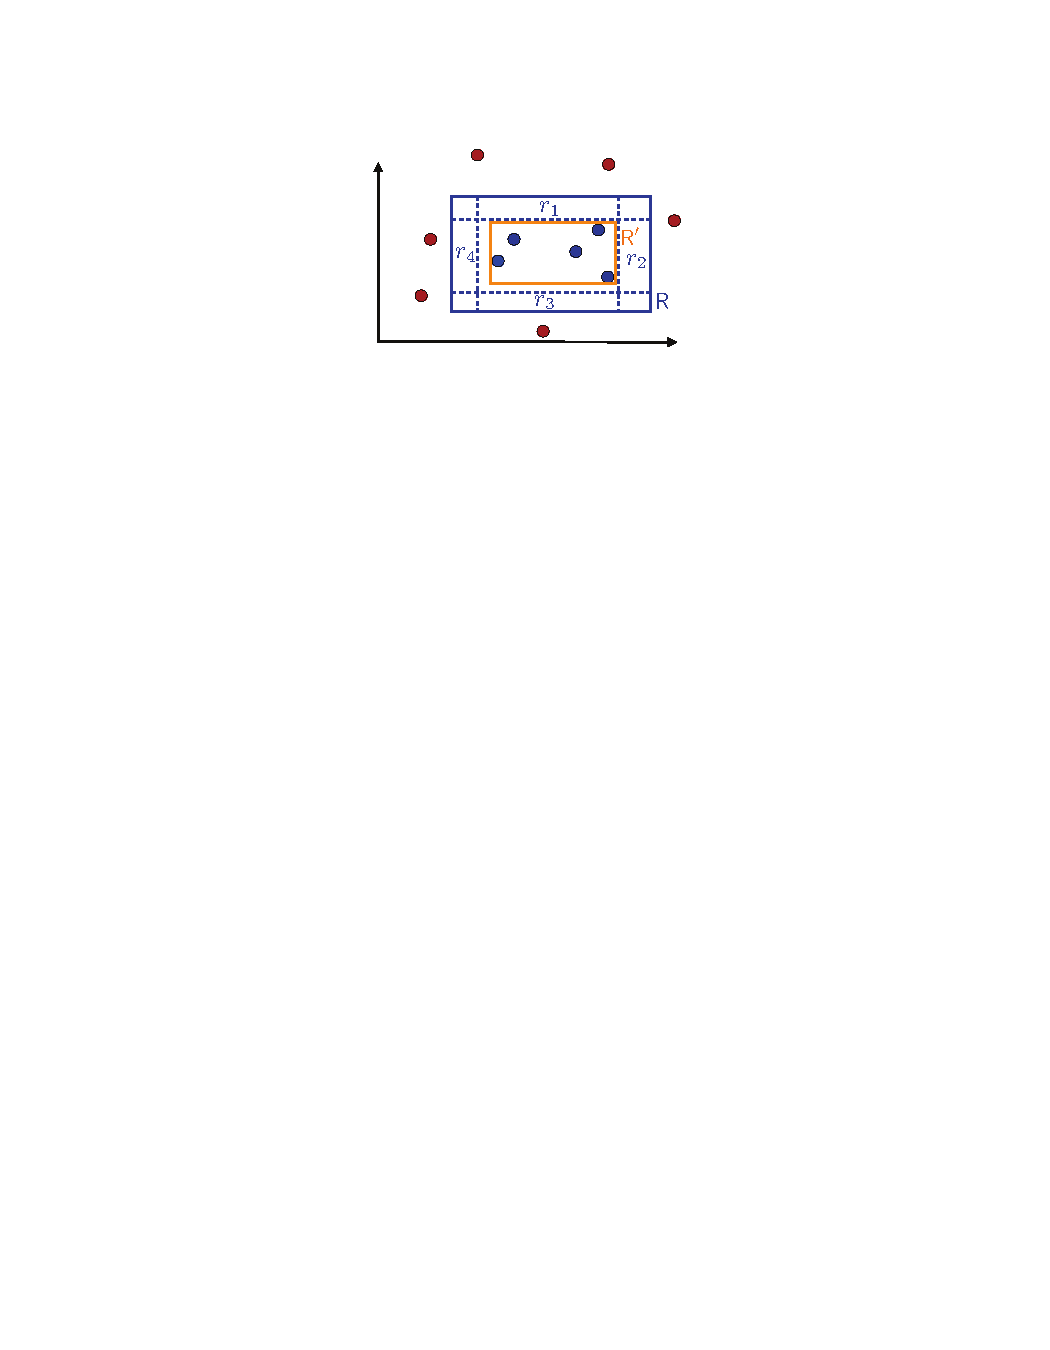
\includegraphics[width=0.5\linewidth]{figures/PAC_rect}
	\caption{Illustration of rectangle $R$ and ``RIG'' regions. \label{fig:pca}}
\end{figure}

See Fig.~\ref{fig:pca}, consider the algorithm $\cA$ finds the smallest rectangle $R'$ containing all positive points. \footnote{This figure is taken from M. Mohri, Foundations of Machine Learning, 2018} We will show that $\cA$ can learn any concept of $R \in \cC$.
\begin{theorem}[Axis-aligned Rectangles are PCA Learnable] Given a dataset with $n$ points, for any $\delta > 0, \epsilon > 0$, to ensure that $p(\cR(R') > \epsilon) \leq \delta$, we can impose a constraint that
$$
 n \geq \mathrm{poly}(1/\epsilon, 1/\delta, \mathrm{size}(R')=4) = \frac{4}{\epsilon} \log \frac{4}{\delta}.
$$
\end{theorem}
\begin{proof}
	Given a prediction $R'$, its risk $\cR(R')$ is the sum of probability of false negative and false positive. More precisely,
	\begin{equation}
		\cR(R') = p\left( \underbrace{(R - R')}_{\text{false neg.}}\ \cup\ \underbrace{(R' - R)}_{false pos.} \right) = p(R - R').
	\end{equation}
	We define four stripes of the $R$, $r_1, r_2, r_3, r_4$, as shown in Fig.~\ref{fig:pca}. Each of the stripe has probability at least $\epsilon / 4$. If the risk exceed $\epsilon$, then $R'$ does not hit at least one of the stripes. We can write,
	\begin{align}
		p(\cR(R') \geq \epsilon) & \leq p_D\left(\bigcup_{i \leq 4} R' \cap r_i = \emptyset\right) \\
		& \leq \sum_{i \leq 4} p_D(R' \cap r_i = \emptyset) \\
		& \leq 4 (1 - \epsilon / 4)^n \\
		& \leq 4 \exp{(-n \epsilon / 4 )}. \qquad\qquad  (1 - x \leq e^{-x})
	\end{align}
To ensure $p(\cR(R') \geq \epsilon) \leq \delta$, we have
\begin{equation}
	4 \exp{(-n \epsilon / 4 )} \leq \delta \ \Longleftrightarrow \ n \geq \frac{4}{\epsilon} \log \frac{4}{\delta}
\end{equation}
\end{proof}             

\section{VC Dimension}
In Vapnik–Chervonenkis theory, the Vapnik–Chervonenkis (VC) dimension is a measure of the capacity (complexity) of a set of functions that can be learned by a \textbf{binary} classification algorithm. 
\begin{definition}
	VC dimension of $\cH$ is defined as the cardinality of the largest set of points on $\cH$ that the algorithm can shatter.
\end{definition}

\begin{table}[h]
{\setstretch{1.25}
\caption{Some interesting examples of VC dimension.}
\begin{tabular}{p{5.8cm} p{6.5cm} p{1.4cm}}
\toprule
	\textbf{Classifier} &  & \textbf{VC-dim} \\
	\midrule
stump classifier & $(-\infty, a]$, $a \in \R$  & $1$   \\
all intervals in $\R$ & $\{[a, b] \mid a, b \in \R \}$  & $2$   \\
all unions of $k$ intervals in $\R$  & $\{\bigcup_{i=1}^k [a_i, b_i] \mid a_i, b_i \in \R \}$ & $2k$  \\
all half-planes in $\R^2$ & $\{(x, y) \mid ax + by + c \geq 0, a, b, c \in \R \}$ & $3$  \\
all convex polygons in $\R^2$ & - & $\infty$ \\
all convex polygons with at most $k$ vertices in $\R^2$ & - & $2k + 1$ \\
\bottomrule
\end{tabular}
}
\end{table}


\section{Concentration Inequalities}
\begin{theorem}[Markov Inequality] Let $X$ be a non-negative random variable. Then
\begin{equation}
	p(X \geq \epsilon) \leq \frac{\EE[X]}{\epsilon}
\end{equation}
\end{theorem}
\begin{theorem}[Hoeffding inequality]
Let $X_1 , . . . , X_m$ be independent random variables with $X_i$ taking values in $[a_i, b_i]$ for all $i \in [m]$. Then, for any $\epsilon > 0$, the following inequalities hold for $S_m = \sum_{i=1}^m X_i$:
\begin{align}
	p(S_m - \EE[S_m] \geq \epsilon) \leq \exp\left( \frac{-2\epsilon^2}{\sum_{i=1}^m (b_i - a_i)^2} \right) \\
	p(S_m - \EE[S_m] \leq -\epsilon) \leq \exp\left( \frac{-2\epsilon^2}{\sum_{i=1}^m (b_i - a_i)^2} \right) 
\end{align}
\end{theorem}

\begin{theorem}[McDiarmid inequality]
Let $X_1, \cdots , X_m \in \mathcal{X}^m$ be a set of $m \geq 1$ independent random variables and assume that there exist $c_1 , \cdots , c_m > 0$ such that $f : \mathcal{X}^m \rightarrow \R$ satisfies the following conditions:	
$$|f(x_1,...,x_i,...,x_m) - f(x_1,...,x'_i,...x_m)|\leq c_i, $$
for all $i \in [m]$ and any points $x_1,...,x_m, x'_i \in \mathcal{X}$. Let $f(S)$ denote $f(X_1,...,X_m)$, then, for all $\epsilon > 0$, the following inequalities hold:
\begin{align}
	p(f(S) - \EE[f(S)] \geq \epsilon) \leq \exp\left( \frac{-2\epsilon^2}{\sum_{i=1}^m c_i^2} \right) \\
	p(f(S) - \EE[f(S)] \leq -\epsilon) \leq \exp\left( \frac{-2\epsilon^2}{\sum_{i=1}^m  c_i^2} \right) 
\end{align}
\end{theorem}
Note that \textit{Hoeffding inequality} is a special instance of \textit{McDiarmid inequality} where $f$ is defined by $f(S) = \frac{1}{m}\sum_{i=1}^m x_i$.
                                                                                                                                                                                                                                                                                                                                                                                                                                                                                                                                  
                                                                                                                                                                                                                                                                                                                                                                                                                                                                                                                                                                                                                                                                                                                                                                                                                                                                                                                                                                                                                                                                                                                                                                                                                                                                                                                                                                                    
%	
%	\newpage
%	\chapter{Exercise}
%	\section{Exercise 8} 

\end{document}